
\chapter{Generating Descriptions With Top-Down Spatial Knowledge}
\chaptersource{Mehdi Ghanimifard and  Simon Dobnik.}{What Goes Into A Word: Generating Image Descriptions With Top-Down Spatial Knowledge.}{In Proceedings of the 12th International Conference on Natural Language Generation. 2019.}

\paragraph{Abstract}
Generating grounded image descriptions requires associating linguistic units with their corresponding visual clues.
A common method is to train a decoder language model with attention mechanism over convolutional visual features. %
Attention weights align %
the stratified visual features %
arranged by their location with tokens, most commonly words, in the target description.
However, %
words such as %
spatial relations (e.g. \emph{next~to} and \emph{under}) are not directly referring to geometric arrangements of pixels but to complex geometric and conceptual representations.
The aim of this paper is to evaluate what representations facilitate generating image descriptions with spatial relations and lead to better grounded language generation. %
In particular, we investigate the contribution of four different representational modalities in generating relational referring expressions:
(i) (pre-trained) convolutional visual features, (ii) spatial attention over visual features, (iii) top-down geometric relational knowledge between objects, and (iv) world knowledge captured by contextual embeddings in language models.


\section{Introduction}\label{inlg2019:sec:introduction}

Spatial recognition and reasoning are essential bases for visual understanding.
Automatically generating descriptions of scenes
involves both recognising objects and their spatial configuration.
This project follows up on recent attempts to improve language
generation and understanding %
in terms of using spatial modules in the fusion of vision and
language
\cite{xu2015show,johnson2016densecap,lu2017knowing,hu2017modeling,anderson2018bottom} (see also %
Section~\ref{inlg2019:sec:related_works}).

Generating spatial descriptions is an important part of the image
description task which requires
several types of knowledge obtained from different modalities: %
 (i) invariant visual clues for object identification,
 (ii) geometric configuration of the scene representing relations between objects relative to the size of the environment %
 (iii) object-specific functional relations that capture interaction between them and are formed by our knowledge of the world %
 for example \emph{an umbrella is over a man} is true if the referring
umbrella serves its function, protecting the man from the rain \cite{coventry2001interplay}, and
 (iv) for projective relations (e.g. ``to the left of'' and ``above'') but not topological relations (e.g. ``close'' and ``at''), the frame of reference which can be influenced from other modalities such as scene attention and dialogue interaction %
 \cite{Dobnik:2015aa}.
 Work in cognitive psychology \cite{logan1994spatial,logan1995linguistic} argues that while object identification may be pre-attentive, identification of spatial relations is not and is accomplished by a top-down mechanisms of attention after the objects have been identified. It is also the case that we do not identify all possible relations between objects but only those that are attended by such top-down mechanisms considering different kinds of high-level knowledge.

Experiments on training neural recurrent %
language models in a bottom-up fashion from data\footnote{
  A bottom-up learning acquires higher level representations from examples of local features rather than using an external procedure to extract them. %
  See also Section~\ref{inlg2019:sec:related_works}.
}
demonstrated that spatial relations are frequently not learned to be grounded in visual inputs
\cite{lu2017knowing,tanti2018quantifying,ghanimifard2018knowing}
which has been attributed
to the design choices of these models that primarily focus on
identification of objects \cite{kelleher2017what}.
Therefore, targeted integration of different modalities is required to
capture the properties from (i) to (iv).  
We can do this top-down	%
\cite{anderson2018bottom,hu2017modeling,liu2017attention}.  
However,
it is not immediately obvious \emph{what} kind of top-down spatial
knowledge will benefit the bottom-up models most. Therefore, in this
paper we investigate the integration of different kind of top-down
spatial knowledge beyond object localisation represented as features with the bottom-up neural
language model.


















The paper is organised as follows.
In Section~\ref{inlg2019:sec:generating_locative_expressions}, we discuss how
spatial descriptions are constructed and what components are required
to generate descriptions. In Section~\ref{inlg2019:sec:neural_net_design}, the
neural networks' design is explained. In Section~\ref{inlg2019:sec:dataset}, we
explain what dataset is used for this study, what pre-processing
was applied on it and how the models are trained. Then the experiments and evaluation results are
presented in Section~\ref{inlg2019:sec:evaluation}. The related work in relation to our methods and findings is discussed %
in Section~\ref{inlg2019:sec:related_works}. %
The conclusion is
given in Section~\ref{inlg2019:sec:conclusion}.


\section{Generating Spatial Descriptions} %
\label{inlg2019:sec:generating_locative_expressions}

When describing a scene, there are several ways to construct spatial
descriptions referring to objects and places and their relation with
each other.  A spatial description has three parts: a \textsc{target}
and a \textsc{landmark} referring to objects or places and a
\textsc{relation} denoting the location of the target in relation to
the landmark \cite{logan1996computational}.\footnote{Sometimes these are also known as \emph{referent} and \emph{relatum} \cite{Miller-JohnsonLaird:1976}, \emph{figure} and \emph{ground} \cite{Talmy:1983} or \emph{the located object} and \emph{the reference object} \cite{herskovits1986language,Gapp:1994:BasicMeanings,Dobnik:2009dz}.} These are in the example in
Figure~\ref{inlg2019:fig:data_example} as follows:

\noindent There~is~$\underbracket{a~teddy~bear}_{\textsc{Target}}~\underbracket{partially~under}_{\textsc{Relation}}~\underbracket{a~go~cart}_{\textsc{Landmark}}$.
\begin{figure}[tb]
	\begin{minipage}{\columnwidth}
	\centering
	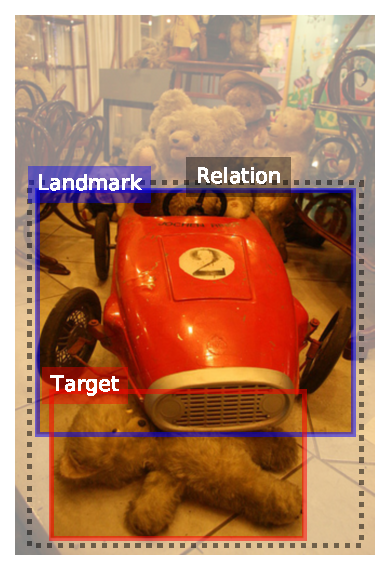
\includegraphics[width=0.4\columnwidth]{studies/inlg2019/figures/2318741.pdf}\\
	$\langle$ ``{\color{red} teddy bear}", ``partially under", ``{\color{blue} go cart}"$\rangle$
	\caption{$\langle$\textsc{target}, \textsc{relation}, \textsc{landmark}$\rangle$ annotation of bounding boxes in VisualGenome 2318741\protect\footnote{\citet{vg2318741}: CC BY-SA 2.0.} }
	\label{inlg2019:fig:data_example}
	\end{minipage}
\end{figure}

\noindent Therefore generating such description requires
(a) identification of objects and their locations:
the target is what we want to describe
and the landmark is what we will relate the target to;
the salience of the landmark is important for the hearer.
(b) Grounding of the relation in geometric space:
the spatial relation is expressed relative to the landmark which
grounds a 3-dimensional coordinate system; furthermore, for projective
relations, the coordinate system is aligned with the orientation of
the external viewpoint which determines the frame of
reference \cite{Maillat:2003}. (Viewpoint may also be the landmark object itself in which
case the coordinate system is oriented in the same way as the
landmark).
(c) Grounding in function:
a spatial relation may be selected also based on the functional
properties between target and landmark objects,
e.g. the difference between ``\textit{the teapot is over the
cup}" and ``\textit{the teapot is above the cup}" \cite{coventry2001interplay}.

Generating spatial descriptions requires knowing the intended target object
and how we want to convey its location to the listener.  The bottom-up
approach in image captioning is focused on learning the salience of
objects and events to generate captions expressed in the dataset (e.g. \citet{xu2015show}).  The combination of bottom-up and
top-down approaches for generating descriptions %
use modularisation in order to improve the generation of descriptions of different kind (e.g. \citet{you2016image}). %
However, as we have seen in the preceding discussion, the generation of
spatial descriptions requires a highly specific geometric knowledge.
How is this knowledge approximated by the bottom-up models?  To what
degree can we integrate this knowledge with the top-down models?  In this
paper, we investigate these questions in a language generation task by comparing
different variations of included top-down spatial knowledge.
More specifically, for each image, we generate a description
for every pair of objects that are localised in the image.
We consider a variety of top-down spatial knowledge representations about objects
as inputs to the model:
(a) explicit object localisation and extraction of visual features;
(b) explicit identification of the target-landmark by specifying their order in the feature vector;
and (c) explicit geometric representation of objects in a 2D image. %
We investigate the contribution of each of these sets of features to generation of image descriptions. %




\section{Neural Network Design}\label{inlg2019:sec:neural_net_design}

Our method is to add step-by-step modules and configurations to the network %
providing different kind of top-down knowledge in Section~\ref{inlg2019:sec:generating_locative_expressions} and investigating the performance of such configurations.
There are several design choices with small effects on the performance but costly in terms of parameter size \cite{tanti2018put}.
Therefore, if there is no research question related to that choice, we take the simplest choice as reported in the previous work such as \cite{lu2017knowing,anderson2018bottom}.
We
use the following configurations: %

\begin{enumerate}[nosep]
	\item Simple bottom-up encoder-decoder; %
	\item Bottom-up object localisation with attention;
	\item Top-down object annotated localisation;
	\item Top-down target and landmark assignment;
	\item Two methods of top-down representation of geometric features ($\bm{s}$-features).
\end{enumerate}
These five %
configurations %
give us 10 variations of the model design as shown in Table~\ref{inlg2019:tab:models}. %
\begin{table*}[htb]
	\centering
	\scriptsize
	\begin{tabular}{|l|l|l|l|l|}
		\hline
		 Model name & Regions Of Interest & \textsc{target}-\textsc{landmark} & $\bm{s}$-features & Architecture \\
		\hline
		$simple$     & - & - & - & Figure~\ref{inlg2019:fig:architectures}a \\
		\hline
		$bu49$       & Bottom-up ($7\mathrm{x}7$ grid) & Bottom-up attention & - & Figure~\ref{inlg2019:fig:architectures}b \\
		$bu49+mask$  & Bottom-up ($7\mathrm{x}7$ grid) & Bottom-up attention & Multi-hot 98 & Figure~\ref{inlg2019:fig:architectures}c \\
		$bu49+VisKE$ & Bottom-up ($7\mathrm{x}7$ grid) & Bottom-up attention & Dense 11 & Figure~\ref{inlg2019:fig:architectures}c \\
		\hline
		$td$         & Top-down (2 bbox) & Bottom-up attention & -    & Figure~\ref{inlg2019:fig:architectures}d \\
		$td+mask$    & Top-down (2 bbox) & Bottom-up attention & Multi-hot 98  & Figure~\ref{inlg2019:fig:architectures}e \\
		$td+VisKE$   & Top-down (2 bbox) & Bottom-up attention & Dense 11 & Figure~\ref{inlg2019:fig:architectures}e \\
		\hline
		$td~order$         & Top-down (2 bbox) & Top-down assign. & - & Figure~\ref{inlg2019:fig:architectures}d \\
		$td~order+mask$    & Top-down (2 bbox) & Top-down assign. & Multi-hot 98 & Figure~\ref{inlg2019:fig:architectures}e \\
		$td~order+VisKE$   & Top-down (2 bbox) & Top-down assign. & Dense 11 & Figure~\ref{inlg2019:fig:architectures}e \\
		\hline
	\end{tabular}
	\vspace{0.5em}
	\caption{The 10 variations of the neural network  model after incrementally adding modules and features.%
	}
	\label{inlg2019:tab:models}
\end{table*}
A detailed definition of each module is given in the Appendix~\ref{appendix:models} in the supplementary material.

\paragraph{Generative language model}
We use a simple forward recurrent neural model with cross-entropy loss in all model configurations.

\paragraph{Simple encoder-decoder}
An encoder-decoder architecture without spatial attention shown in  Figure~\ref{inlg2019:fig:architectures}a and similar to \cite{vinyals2015show} is the simplest baseline for %
fusing vision and language.
The input to the model is an image and the start symbol $<s>$ of a description and the output is produced by the language model decoder.
The embeddings are randomly initialised and learned as a parameter set of the model.
The visual vectors are produced by a pre-trained ResNet50 \cite{he2016deep}.
A multi-layer perceptron module ($F_v$ in Figure~\ref{inlg2019:fig:visual_finetune_a}) is used to fine-tune the visual features.

\begin{figure}[htb]
	\begin{minipage}{\columnwidth}
		\centering
		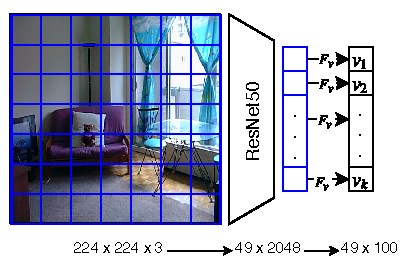
\includegraphics[scale=0.75]{studies/inlg2019/figures/general_visual_features.pdf}
	\end{minipage}%
	\caption{Visual features are obtained from the pre-trained ResNet50, then translated to a low dimensional vector with a dense layer $F_v$. 
	}
	\label{inlg2019:fig:visual_finetune_a}
\end{figure}

\paragraph{Bottom-up localisation}
With visual feature representing all regions of the image as in Figure~\ref{inlg2019:fig:visual_finetune_a}, the attention mechanism is used %
as a localisation module. %
We generalised %
the adaptive attention introduced in \cite{lu2017knowing} to be able to fuse the modalities.
As shown in Figure~\ref{inlg2019:fig:architectures}b, the interaction between the attention mechanism and the language model is more similar to \cite{anderson2018bottom}: two layers of stacked LSTM, the first stack ($\mathrm{LSTM}_a$) to produce the features for the attention model and the second stack ($\mathrm{LSTM}_l$) to produce contextualised linguistic features which are fused with the attended visual features.
This design is easier to extend with additional top-down vectors.

\begin{figure*}[th]
	\begin{minipage}{.19\textwidth}
		\centering
		\vspace{7mm}
		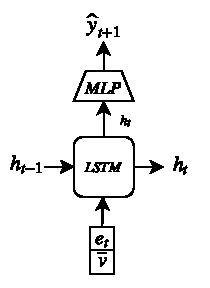
\includegraphics[scale=0.65]{studies/inlg2019/figures/simple_no_attention_no_location.pdf} \\
		\vspace{4mm}
		(a)
	\end{minipage}%
	\begin{minipage}{.20\textwidth}
		\centering
		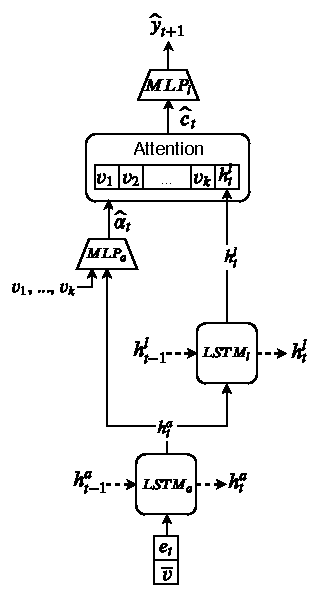
\includegraphics[scale=0.43]{studies/inlg2019/figures/bottom-up.pdf}\\
		(b)
	\end{minipage}%
	\begin{minipage}{.20\textwidth}
		\centering
		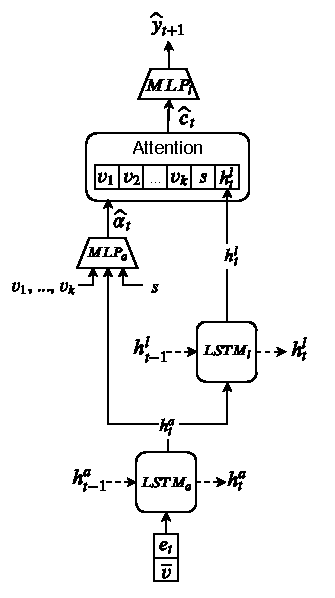
\includegraphics[scale=0.43]{studies/inlg2019/figures/bottom-up+s.pdf}\\
		(c)
	\end{minipage}%
	\begin{minipage}{.20\textwidth}
		\centering
		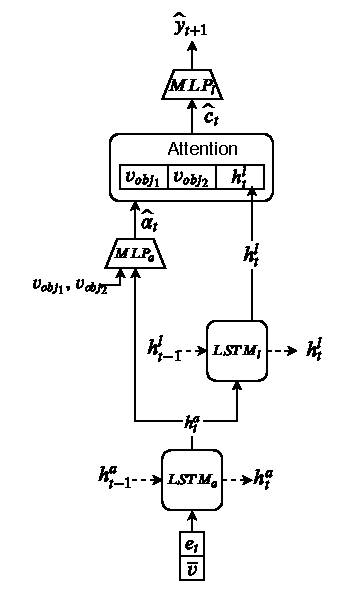
\includegraphics[scale=0.43]{studies/inlg2019/figures/top-down.pdf} \\
		(d)
	\end{minipage}%
	\begin{minipage}{.20\textwidth}
		\centering
		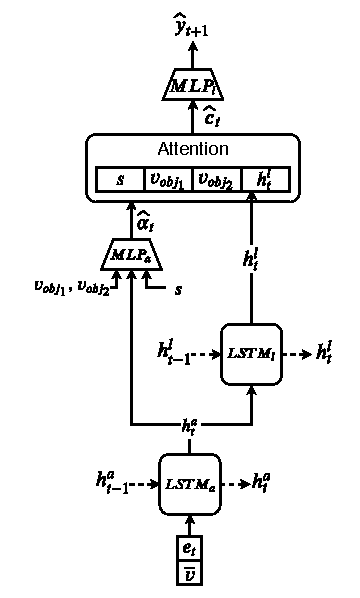
\includegraphics[scale=0.43]{studies/inlg2019/figures/top-down+s.pdf} \\
		(e)
	\end{minipage}%
	\caption{Five architectures: (a) simple encoder-decoder ($simple$). (b) bottom-up localisation with adaptive attention on 49 regions ($bu49$). (c) bottom-up localisation with explicit spatial vectors of the bounding boxes $bu49+mask$/$bu49+VisKE$. (d) top-down localisation with attentions on two bounding boxes ($td$). (e) top-down localisation augmented with explicit spatial vectors of the bounding boxes ($td+mask$/$td+VisKE$).}
	\label{inlg2019:fig:architectures}
\end{figure*}


\paragraph{Top-down localisation}
Unlike the bottom-up unsupervised localisation, the top-down method includes a provision of a list regions of interest (ROI) from external procedures.
For example, the region proposals can come from another bottom-up task as in \cite{anderson2018bottom,johnson2016densecap} which use a Faster R-CNN \cite{ren2015faster} to extract possible regions of interest from the ConvNets regions in Figure~\ref{inlg2019:fig:visual_finetune_a}.
Here, as shown in Figure~\ref{inlg2019:fig:visual_finetune_b} we use the bounding box annotations of objects in images as the top-down localisation knowledge and then  extract ResNet50 visual features from these regions.
In the first stage the top-down visual representation only proposes visual vectors of the two objects in a random order without their spatial role as targets and landmarks in the descriptions. The model is shown in Figure~\ref{inlg2019:fig:architectures}d.

\begin{figure}[htb]
	\begin{minipage}{\linewidth}
		\centering
		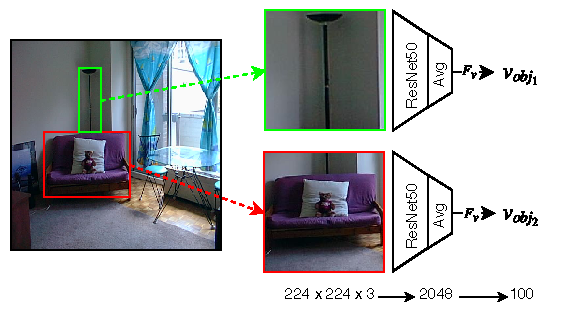
\includegraphics[scale=0.75]{studies/inlg2019/figures/objects_visual_features.pdf}
	\end{minipage}%
	\caption{
		Top-down localisation of objects with bounding boxes whose visual features are extracted and translated to lower dimensions with $F_v$.
	}
	\label{inlg2019:fig:visual_finetune_b}
\end{figure}

\paragraph{Top-down target-landmark assignment}

In the second iteration of the top-down localisation module we assign semantic roles to regions as targets and landmarks.
This is directly related to localisation as spatial relations are asymmetric.
	We encode this top-down knowledge by fixing the order of the regions in the feature vector. The first object is the target and the second object is the landmark. Otherwise, the model is the same as in the previous iteration shown in Figure~\ref{inlg2019:fig:architectures}d.

\paragraph{Top-down geometric features}
The localisation procedure of objects discussed previously does not provide any geometric information about the relation between the two regions. %
However, top-down geometric features are required for grounding spatial relations %
where the location of the target object is expressed relative to the landmark.
For example, a simple (but by no means sufficient) geometric relation between two bounding boxes can be represented by an arrow from the centre of one bounding box to the centre of the other %
and by ordering the information about bounding boxes in the feature vector as in the previous model to encode target-landmark asymmetry. %
The network architecture of the model with top-down geometric features expressing relations between the objects is shown in Figure~\ref{inlg2019:fig:architectures}e.
We consider two different representations of the top-down geometric features %
shown in Figure~\ref{inlg2019:fig:spatial}:
Multi-hot mask over 49 vectors independently for target and landmark ($Mask$) over 49 locations (Figure~\ref{inlg2019:fig:spatial}a) and $VisKE$ \cite{sadeghi2015viske} dense representations with 11 geometric features (Figure~\ref{inlg2019:fig:spatial}b) where $dx, dy$ are changes in the coordinates of the centres, %
$ov, ov_1, ov_2$ the overlapping areas (total, relative to the first, and the second bounding box), $h_1, h_2$ heights, $w_1, w_2$ widths and $a_1, a_2$ areas. Note that $Mask$ features provide geometric information about the size and the location of objects relative to the picture frame and $VisKE$ feature provide more detailed geometric information that expresses the relation between the objects. The latter therefore more closely match the features that were identified in spatial cognitive models.
A feed-forward network with two layers ($F_s$) is used to project geometric features into a vector with the same dimensionality as the $F_v$ outputs so that different modalities are comparable
in weighted sum model of attention.


\begin{figure}[htb]
	\begin{minipage}{0.63\linewidth}
		\centering
		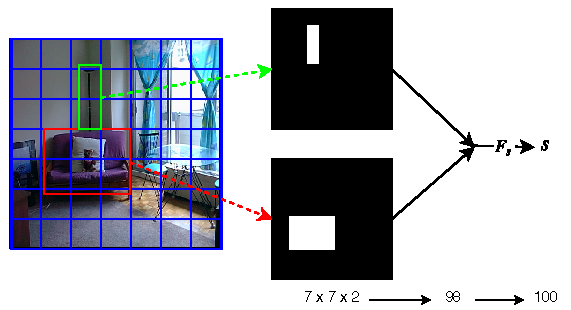
\includegraphics[scale=0.65]{studies/inlg2019/figures/extrinsic_representation_mask.pdf} \\
		(a)
	\end{minipage}%
	\begin{minipage}{0.37\linewidth}
		\centering
		\includegraphics[scale=0.65]{studies/inlg2019/figures/extrinsic_representation_VisKE.pdf} \\
		(b)
	\end{minipage}%
	\caption{
		(a) Each bounding box is converted to a mask of multi-hot vector on 49 regions.
		(b) The geometric relation between the two bounding boxes are represented with features from \cite{sadeghi2015viske}.
	}
	\label{inlg2019:fig:spatial}
\end{figure}





\section{Dataset and Training}\label{inlg2019:sec:dataset}

We %
use the relationship dataset in Visual Genome \cite{krishna2017visual} which is
a collection of referring expressions represented as triplets $\langle \mathrm{subject}, \mathrm{predicate}, \mathrm{object} \rangle$ on 108K images.
Unlike image captioning datasets such as MSCOCO \cite{chen2015microsoft} and Flickr30K \cite{plummer2015flickr30k} where only 5 captions are given for each image, each image in this dataset is annotated with 50 phrases.
The annotators were asked to annotate relations between two given bounding boxes of $\mathrm{subject}$ and $\mathrm{object}$ by freely writing the text for each of the three parts of the annotation.
The bounding boxes %
produced by another annotation procedure which detected objects in the images. %
In total, there are $2,316,104$ annotations of $664,805$ unique triplets, $35,744$ unique labels of subjects and $21,299$ unique labels of objects most of which
consist of multiple tokens.
We omit all repetitions of triplets on each image, this leaves total $1,614,055$ annotations.\footnote{The repetitions include reflexive expressions (e.g. \emph{horse next to horse}), annotations of several objects of the same type (e.g. \emph{cup on table}), and repetitions due to several bounding box annotations of the same objects with different sizes.} %

\paragraph{Spatial relations}
Based on the lists of spatial prepositions in \citep{Landau:1996aa} and
\citep{herskovits1986language}, we have created a dictionary of spatial relations and their possible multi-word variants including their composite forms.
This dictionary contains $7,122$ entries of $235$ relations (e.g. \emph{right} to represent both \emph{on the right hand side of} and \emph{to the right of}). Of these only $202$ are found in Visual Genome dataset covering $79$ spatial relations.
$328,966$ unique triplets in Visual Genome are based on exactly one of these terms which covers $49.4\%$ of all possible relationships.\footnote{Other triplets in Visual Genome also have spatial content.
Some of them %
include modifiers such as \emph{partially under} as in Figure~\ref{inlg2019:fig:data_example} and some of them are descriptions of an event or an action such as \emph{sitting on} and \emph{jumping over}. Some annotated relationships are verbs such as \emph{flying} with less obvious spatial denotation.
The spatial bias in the dataset was studied in \cite{collell2018acquiring}.
The most frequent spatial relation in the dataset is ``\emph{on}" (over 450K instances), the second place is ``\emph{in}" (150K instances), %
then ``\emph{with}", variations of ``\emph{behind}", ``\emph{near}", ``\emph{top}", ``\emph{next}", ``\emph{under}", ``\emph{front}", and ``\emph{by}" (less than 10K instances each).}

\paragraph{Bounding boxes}
Each bounding box is a tuple of 4 numbers $(x, y, w, h)$. We normalise the numbers to the range of $(0,1)$ relative to the image size to create geometric feature vectors (Section~\ref{inlg2019:sec:neural_net_design}).
The image is split into a grid with 7x7 cells to which bounding boxes are mapped, one bounding box potentially covering more than one cell.
With this bounding box granularity, there are exactly $308,330$ possible bounding boxes. However, only $151,974$ are observed in the relationships dataset. The spatial distribution of paired objects reflects how natural pictures are framed and how related objects are understood by annotators.

\paragraph{Pre-processing}

We first removed duplicate %
triplets describing the same image. Then we converted each triplet into a word sequence by concatenating the strings and de-tokenising them with the white space separator.
This produced a corpus with a vocabulary of $26,530$ types with a maximum sequence length of 16 tokens and on average 15 referring expressions per image.
We use 95\% of the descriptions for training and 5\% for validation and testing
(5,230 images with 80,231 triplets).%


\paragraph{Training}\label{inlg2019:sec:implementation}
We use Keras \cite{chollet2015keras} with TensorFlow backend \cite{tensorflow2015-whitepaper} to implement and train all of the neural network architectures in Section~\ref{inlg2019:sec:neural_net_design}.
The models are trained with the Adam optimiser \cite{kingma2014adam} ($\alpha=0.001$, $\beta_1=0.9$, $\beta_2=0.999$) with a batch size of 128 and 15 epochs.

\section{Evaluation}\label{inlg2019:sec:evaluation}
All implementations are available online\footnote{
\url{https://gu-clasp.github.io/generate_spatial_descriptions/}}.
\subsection{Qualitative Examples}
Figure~\ref{inlg2019:fig:data_example2} shows generated descriptions for two
examples of unseen pictures from the test dataset by five models. The
generated word sequence is that with the lowest loss using beam search
with $k=5$. The first example shows exactly how top-down localisation of
objects is important especially if the goal is to refer to specific objects
in the scene. In the second example, the visual features inside the bounding
box are confusing for all 5 models. More examples are in Figure~\ref{inlg2019:fig:data_example2a} in the Appendix.

\begin{figure}[ht!]
	\centering
	\begin{minipage}{0.55\linewidth}
		\centering
		\begin{minipage}{\columnwidth}
			\centering
			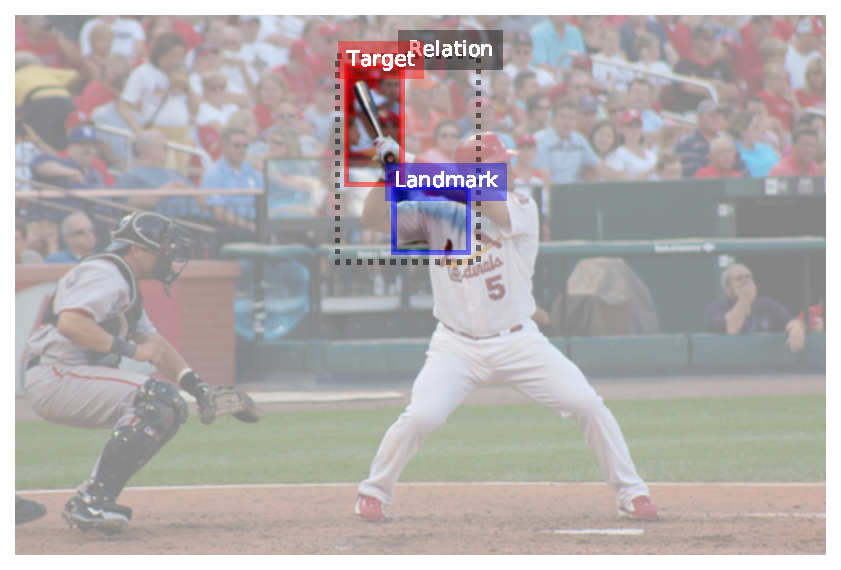
\includegraphics[width=\columnwidth]{studies/inlg2019/figures/2412051_bat_over_shoulder.pdf}\\
			$\langle$ ``{\color{red} bat}", ``over", ``{\color{blue} shoulder}"$\rangle$ \\
		\end{minipage} \\
		\begin{minipage}{\columnwidth}%
			\small
			\begin{tabular}{ll}
				$simple$         & {player} \\
				$bu49$           & {man~wearing~shirt} \\
				$td$             & {bat~in~hand} \\
				$td~order$       & {bat~in~hand} \\
				$td~order+VisKE$ & {bat~in~hand} \\
				\hline
			\end{tabular}
		\end{minipage}
	\end{minipage}\\
	\begin{minipage}{0.55\linewidth}
		\centering
		\begin{minipage}{\columnwidth}
			\centering
			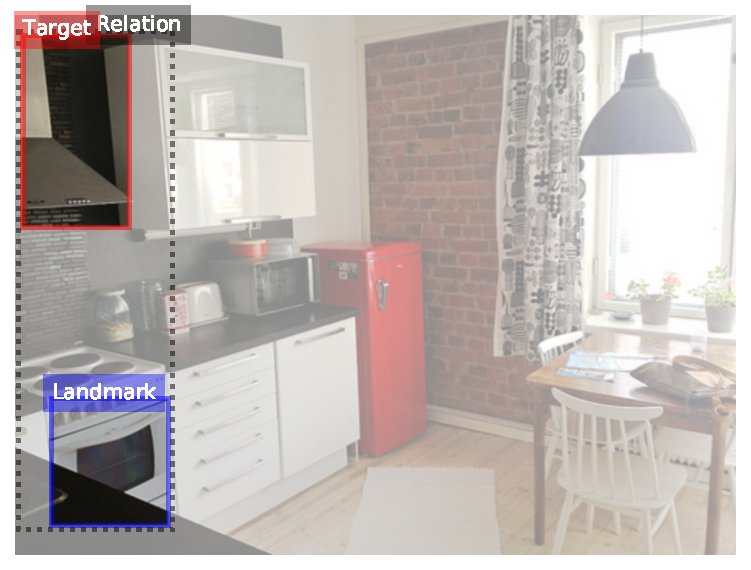
\includegraphics[width=\columnwidth]{studies/inlg2019/figures/2413282_hood_above_oven.pdf} \\
			$\langle$ ``{\color{red} hood}", ``above", ``{\color{blue} oven}"$\rangle$ \\
		\end{minipage} \\
		\begin{minipage}{\columnwidth}%
			\small
			\begin{tabular}{ll}
			$simple$         & {window} \\
			$bu49$           & {pot~on~stove} \\
			$td$             & {oven~has~door} \\
			$td~order$       & {vent~above~sink} \\
			$td~order+VisKE$ & {cabinet~has~door} \\
			\hline
			\end{tabular}
		\end{minipage}
	\end{minipage}
	\caption{From VisualGenome: 
	2412051\protect\footnote{\citet{vg2412051}: CC BY-SA 2.0.}
	2413282\protect\footnote{\citet{vg2413282}: CC BY-NC-SA 2.0.}
	}\label{inlg2019:fig:data_example2}
\end{figure}


\subsection{Overall Model Performance}
\paragraph{Hypothesis}
Top-down spatial knowledge improves the model performance.  We
consider three categories of top-down spatial knowledge: (i) top-down
localisation of regions of interest; (ii) top-down assignment of
semantic roles to regions; and (iii) two kinds of geometric feature
vectors.



\paragraph{Method}
After training the models we evaluate them by calculating the average word level
cross-entropy loss on %
held out instances in the
test set\footnote{Equivalent to log-perplexity of the language model.}. %
We also calculate the loss on descriptions containing specific
spatial relations %
for qualitative understanding of %
the effects of each type of top-down knowledge.

\paragraph{Results}
The overall loss of each model on
the %
unseen descriptions of images is shown in Figure~\ref{inlg2019:fig:loss}.  The
fully bottom-up model with no spatial attention ($simple$) has the
highest
loss. %
The loss in the variations of the model with bottom-up localisation in
$bu49$ is higher than the one in the models with top-down
localisation. %
The models with the top-down assignment of
\textsc{target}-\textsc{landmark} achieves the best
results. %
The effect of top-down geometric features is not significant.


\begin{figure}[ht!]
	\centering
	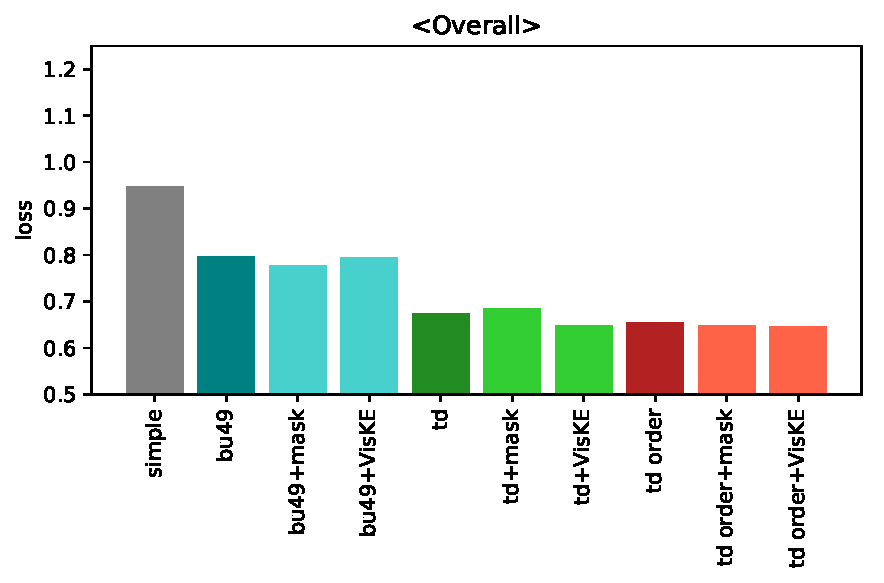
\includegraphics[width=0.6\columnwidth]{studies/inlg2019/figures/results/loss/all.pdf}%
	\caption{Cross-entropy loss of different model configurations on evaluation data.}
	\label{inlg2019:fig:loss}
\end{figure}


Figure~\ref{inlg2019:fig:sp_loss} shows the performance of the models on a selection
spatial relations.

\begin{figure}[ht!]
\begin{minipage}{0.5\columnwidth}
	\centering
	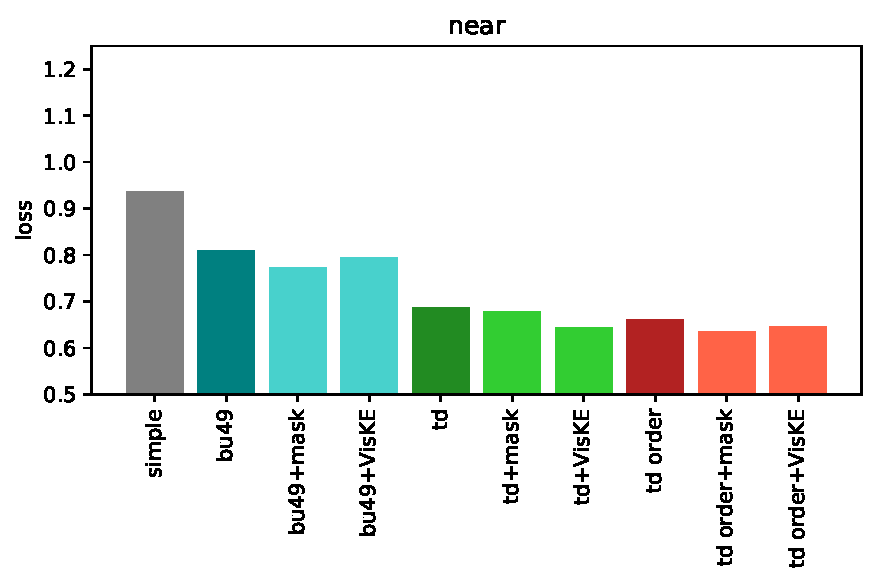
\includegraphics[width=\columnwidth]{studies/inlg2019/figures/results/loss/near.pdf}%
\end{minipage}%
\begin{minipage}{0.5\columnwidth}
	\centering
	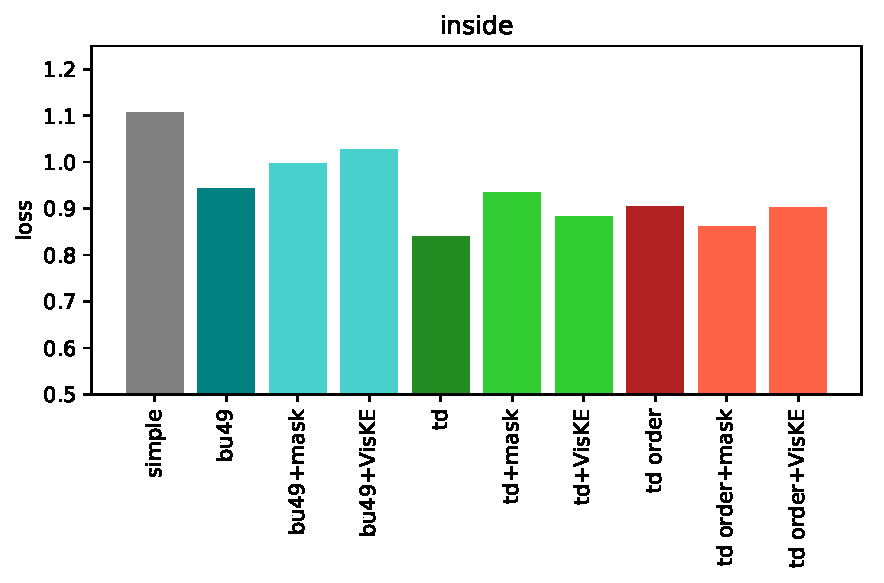
\includegraphics[width=\columnwidth]{studies/inlg2019/figures/results/loss/inside.pdf}%
\end{minipage}\\
\begin{minipage}{0.5\columnwidth}
	\centering
	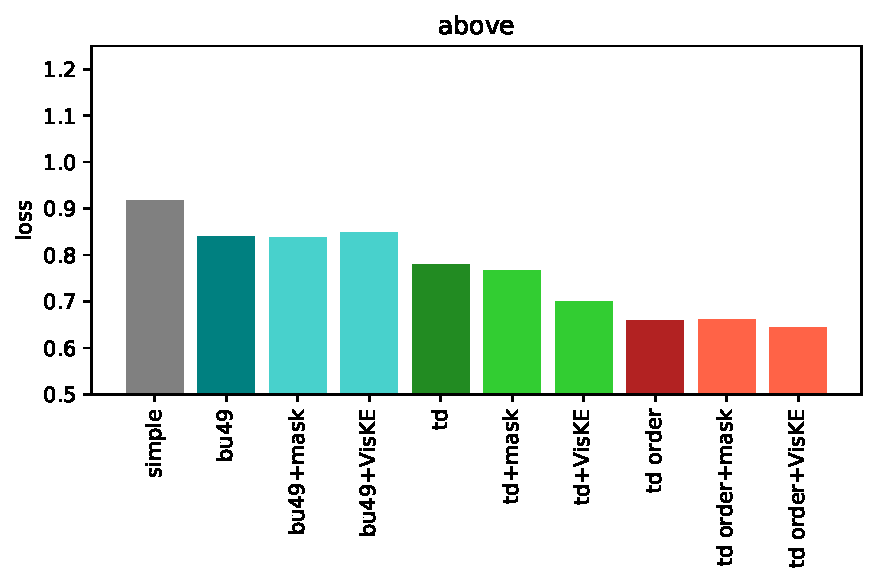
\includegraphics[width=\columnwidth]{studies/inlg2019/figures/results/loss/above.pdf}%
\end{minipage}%
\begin{minipage}{0.5\columnwidth}
	\centering
	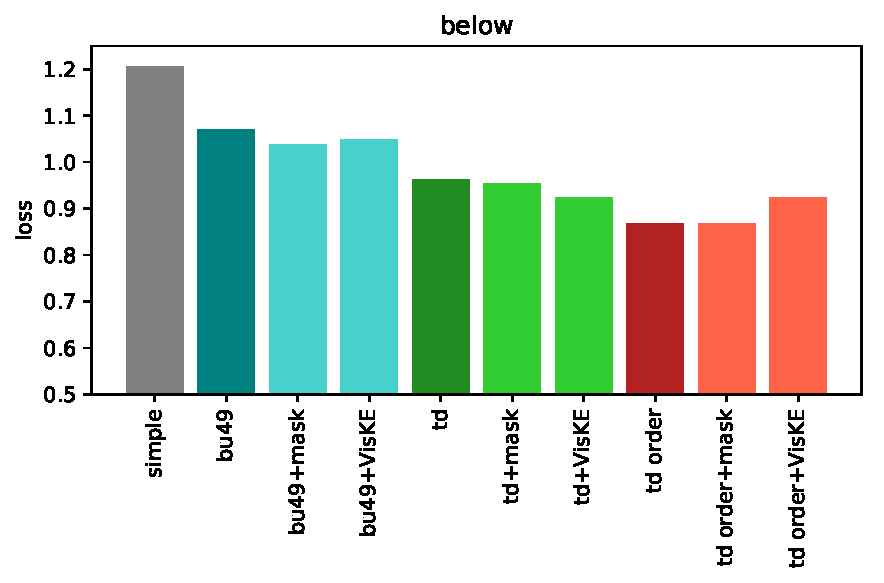
\includegraphics[width=\columnwidth]{studies/inlg2019/figures/results/loss/below.pdf}%
\end{minipage}\\
\begin{minipage}{0.5\columnwidth}
	\centering
	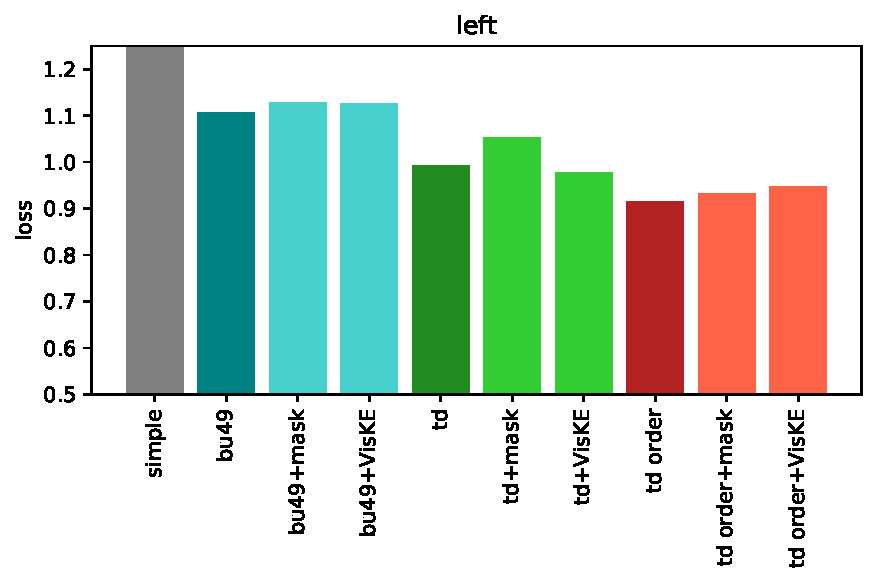
\includegraphics[width=\columnwidth]{studies/inlg2019/figures/results/loss/left.pdf}%
\end{minipage}%
\begin{minipage}{0.5\columnwidth}
	\centering
	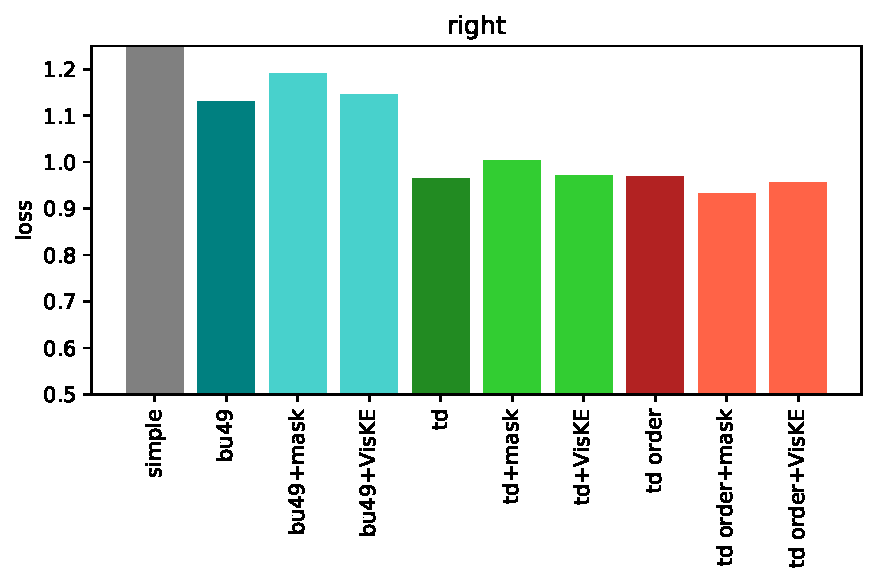
\includegraphics[width=\columnwidth]{studies/inlg2019/figures/results/loss/right.pdf}%
\end{minipage}%
	\caption{Cross-entropy loss of different model configurations on 40 descriptions for each relation: \emph{near}, \emph{inside}, \emph{above} and \emph{below}.}
	\label{inlg2019:fig:sp_loss}
\end{figure}



\paragraph{Discussion}

The top-down localisation ($td$) certainly improves the performance of the language models
compared to purely bottom-up representations.  
However, additional top-down assignment
of \textsc{target}-\textsc{landmark} ($td~order$) 
and their %
additional geometric arrangement of bounding box features ($mask$ and $VisKe$) has a small positive effect on overall performance.
The overall performance is not a representative of how these configurations effect the grounding of spatial relations.
More specifically, the imbalance of certain groups of relations (especially a generally lower proportion of geometrically biased relations such as ``left'' and ``right'' in this dataset and the presence of relations with a minimum spatial content such as \emph{has}, \emph{wearing}) makes it harder to make conclusions about overall performance of the models. %
We further examine two groups of some frequent spatial relations.
The relations such as \emph{inside} and \emph{near} represent one group
and \emph{above} and \emph{below} represent the other.  
Some top-down knowledge (as represented by our features)
is less informative for the first group but is informative for the
second group. 
For example \emph{near} does not require the assignment of  \textsc{target}-\textsc{landmark} roles. %
We observe that $td~order$ is not performing better than $td$.
On the other hand, \emph{inside} is sensitive to \textsc{target}-\textsc{landmark} assignment. However, since the relation is also restricted by a choice of objects (only certain objects can be inside others)  %
their \textsc{target}-\textsc{landmark} assignment may already be inferred without such top-down knowledge from a language model. 
For the second group, the top-down knowledge
about the semantic role of objects is important. 
However, \emph{left} and \emph{right} are among the least  frequent relations in the dataset which is demonstrated by the fact that their descriptions have a higher loss than \emph{above} and \emph{below}.
For these relations the loss of the $simple$ model is much higher than other configurations. 
It can be seen that $td$ is performing better than $bu$ and $td~order$ is contributing over $td$ but geometric features have a lesser effect than identification of semantic roles ($td~order$).



\subsection{Grounding in features}
\paragraph{Hypotheses}
With the aim to evaluate \emph{what} top-down information contributed
to grounding of words we examine the following hypotheses:
\begin{itemize}[noitemsep]
\item[H1] $\bm{s}$-features contribute to predicting spatial relation
  words.
\item[H2] Without top-down \textsc{target}-\textsc{landmark} %
  role assignments to
  each region, 
  attention is uniformly distributed over region choices
  at the beginning of a sequence
  generation.


\end{itemize}


\paragraph{Method}
In order to check the contribution of each feature from different
modalities %
in prediction of each word, we look at the adaptive attention on each
feature at the point of predicting the word\footnote{
In this experiment, we do not check if the estimated likelihood for the correct word is the highest predicted score. 
The generated descriptions may still be acceptable with an alternative spatial relation. Furthermore, in the following analysis we report the attention over semantic roles and not individual words.
}.  Since feature vectors
are not normalised against the number of features of each modality, we
first multiply each attention measure with the magnitude of the
feature vector, and then we normalised it to sum to 1 again:
\begin{equation}\label{inlg2019:eq:nomalised_attention}
\bm{\beta}_{t,f_i} = \frac{\bm{\alpha}_{t,f_i} ||f_i||}{\sum_{j}{\bm{\alpha}_{t,f_j} ||f_j||}}
\end{equation}
\noindent where $t$ refers to the time in the word sequence, and $f_i$
is the feature the attention of which $\bm{\alpha}_{t,f_i}$ is applied
to it. We report the average $\bm{\beta}_{t,f_i}$ over the instances
in the validation dataset.

Figure~\ref{inlg2019:fig:examples} shows $\bm{\beta}$ on two examples in three models.
For each word, the bar chart is divided between four features (in Figure~\ref{inlg2019:fig:architectures}e): (1) target $v_{obj_1}$ (2) landmark $v_{obj_2}$ (3) $\bm{s}$-features for bounding boxes (4) contextualized embeddings $h^l$.
\begin{figure}[ht!]
	\centering
	\begin{minipage}{0.75\linewidth}
		\centering
		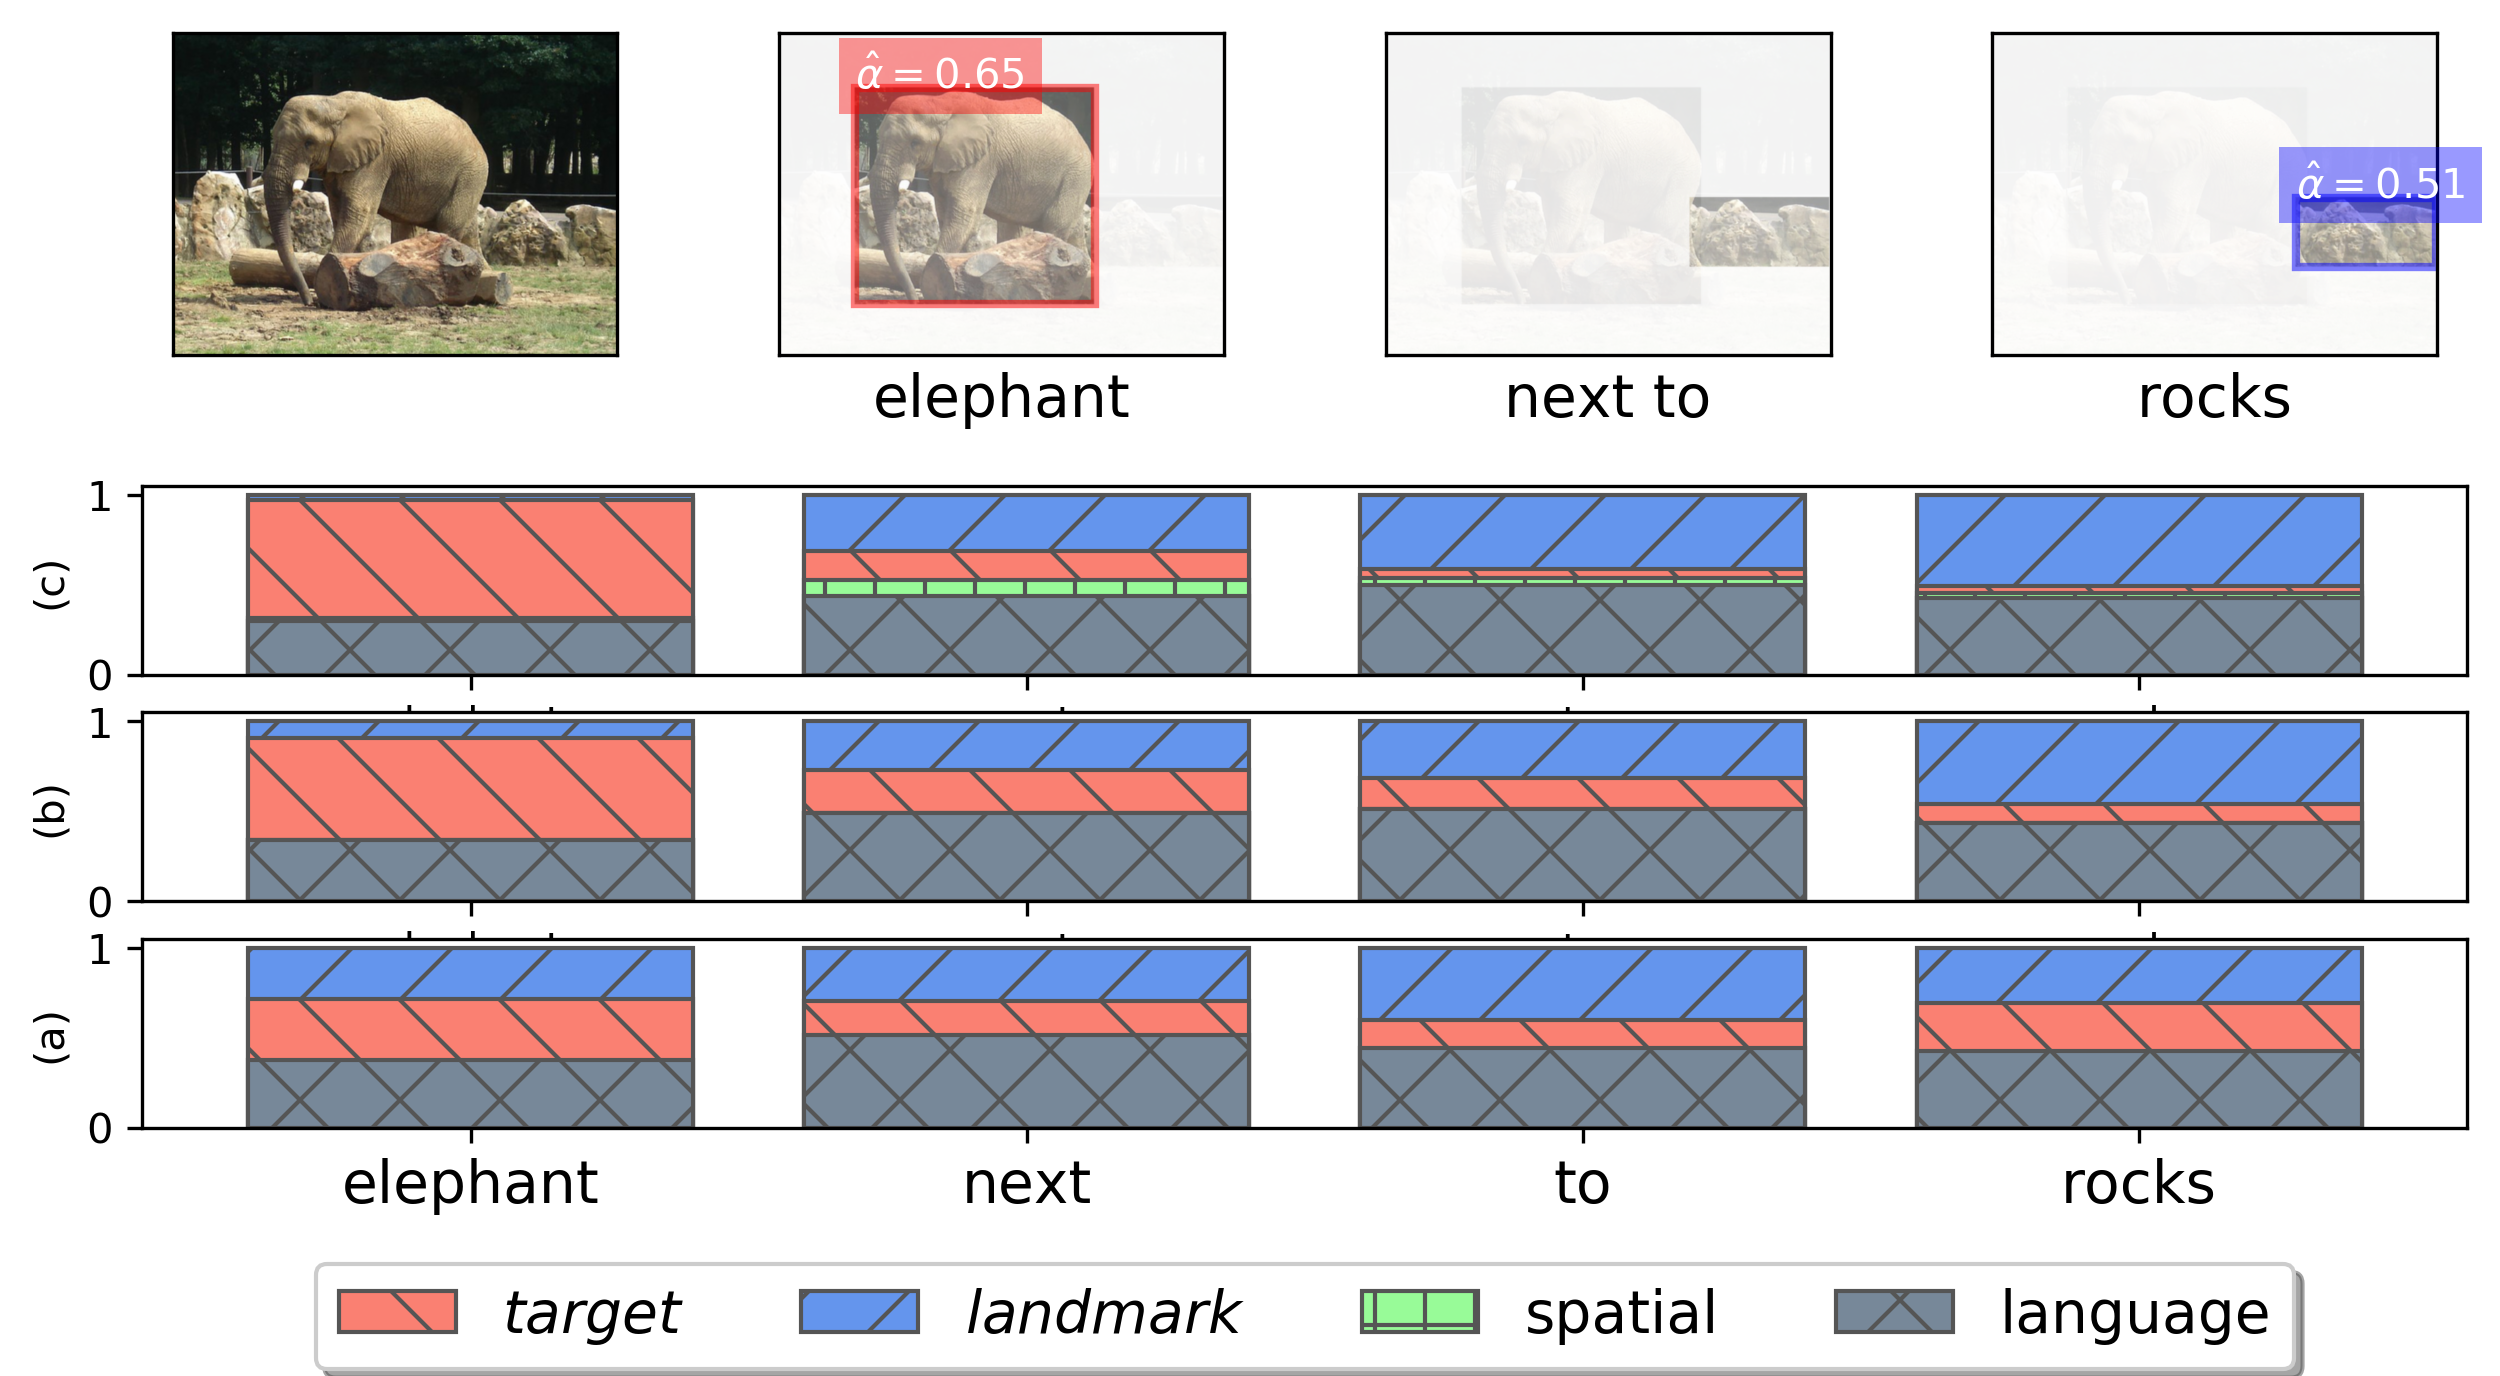
\includegraphics[width=\columnwidth]{studies/inlg2019/figures/results/examples/mix/elephant_next_to_rocks.png}
	\end{minipage}\\
	\begin{minipage}{0.75\linewidth}
	\centering
	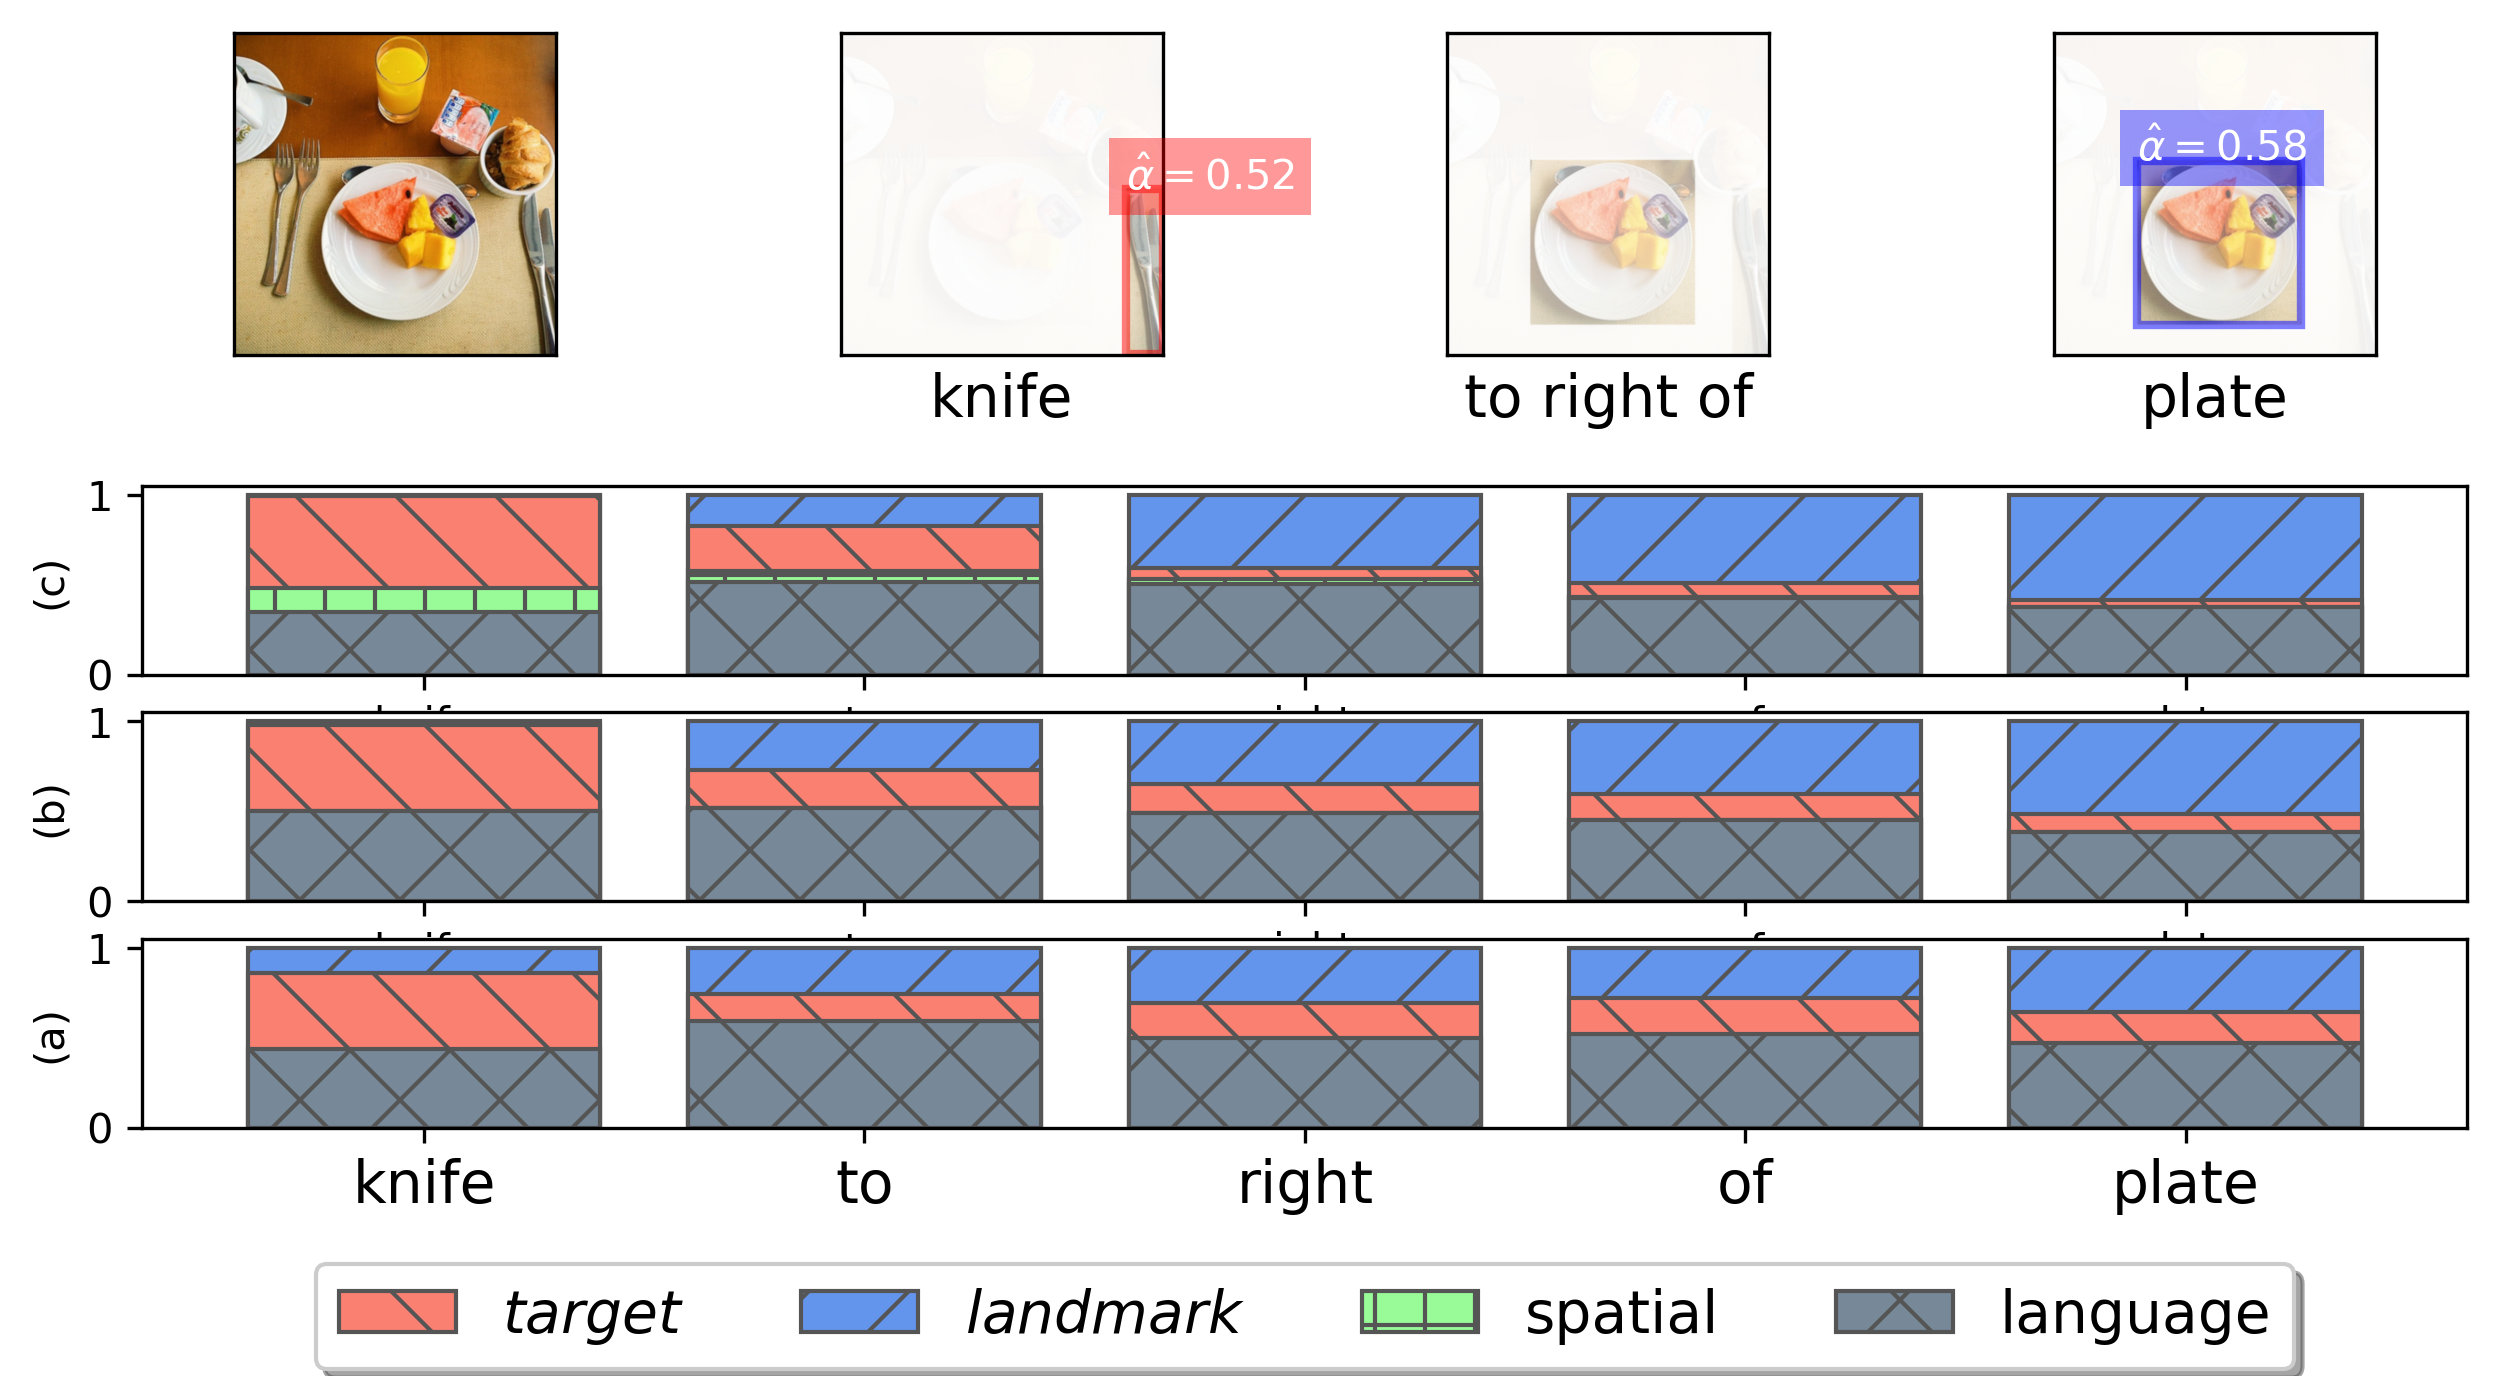
\includegraphics[width=\columnwidth]{studies/inlg2019/figures/results/examples/mix/knife_to_right_of_plate.png}
	\end{minipage}%
	\caption{$\bm{\beta}$ is plotted in bar charts for each word.
		(a) $td~order+VisKE$
		(b) $td+VisKE$
		(c) $td$.
		The values of $\bm{\beta}$ for each word that constitute description referring to each bounding box region is given in images.
	}
	\label{inlg2019:fig:examples}
\end{figure}


After measuring the normalised attention on each feature according to
Equation~\ref{inlg2019:eq:nomalised_attention}, we report the average of
attentions on each token at that time step
of the word sequence. We also %
group the tokens based on their semantic role in the triplets and
report the average $\bm{\beta}$ on these tokens for a given role.


\paragraph{Results} The average of %
attentions over triplets of tokens is plotted in
Figure~\ref{inlg2019:fig:attention_roles}. The behaviour of attentions on word
sequences in the four models in given in
Figure~\ref{inlg2019:fig:attention_trend}.


\begin{figure}[ht!]
	\centering
	\begin{minipage}{0.3\linewidth}
		\centering
		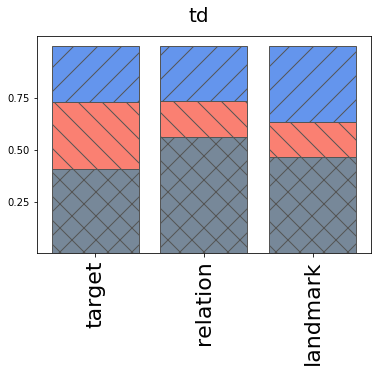
\includegraphics[width=\columnwidth]{studies/inlg2019/figures/results/attentions/models/td.png}\\
	\end{minipage}%
	\begin{minipage}{0.3\linewidth}
		\centering
		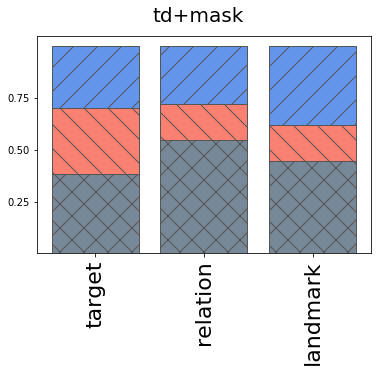
\includegraphics[width=\columnwidth]{studies/inlg2019/figures/results/attentions/models/td+mask.png}\\
	\end{minipage}%
	\begin{minipage}{0.3\linewidth}
		\centering
		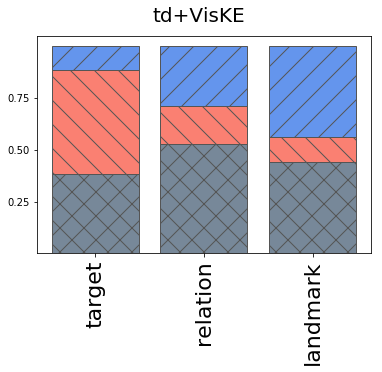
\includegraphics[width=\columnwidth]{studies/inlg2019/figures/results/attentions/models/td+VisKE.png}\\
	\end{minipage}\\
	\begin{minipage}{0.3\linewidth}
		\centering
		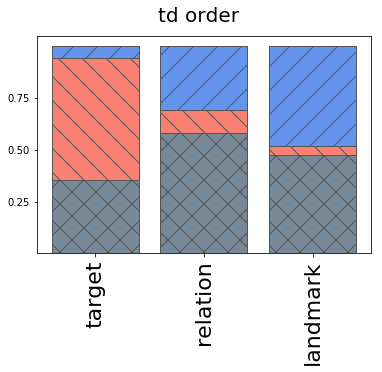
\includegraphics[width=\columnwidth]{studies/inlg2019/figures/results/attentions/models/td_order.png}\\
	\end{minipage}%
	\begin{minipage}{0.3\linewidth}
		\centering
		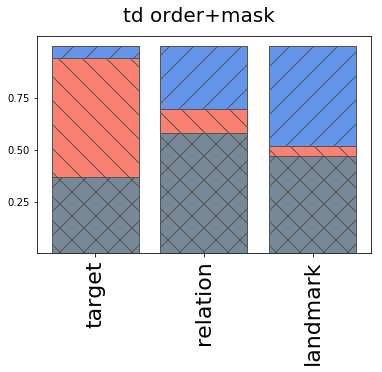
\includegraphics[width=\columnwidth]{studies/inlg2019/figures/results/attentions/models/td_order+mask.png}\\
	\end{minipage}%
	\begin{minipage}{0.3\linewidth}
		\centering
		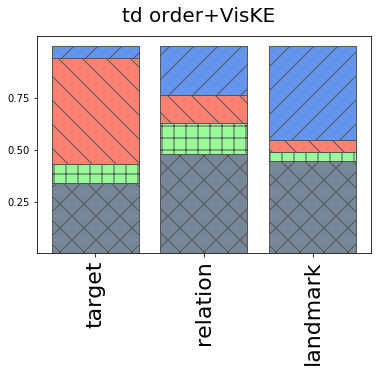
\includegraphics[width=\columnwidth]{studies/inlg2019/figures/results/attentions/models/td_order+VisKE.png}\\
	\end{minipage}\\
	\begin{minipage}{0.9\linewidth}
		\centering
		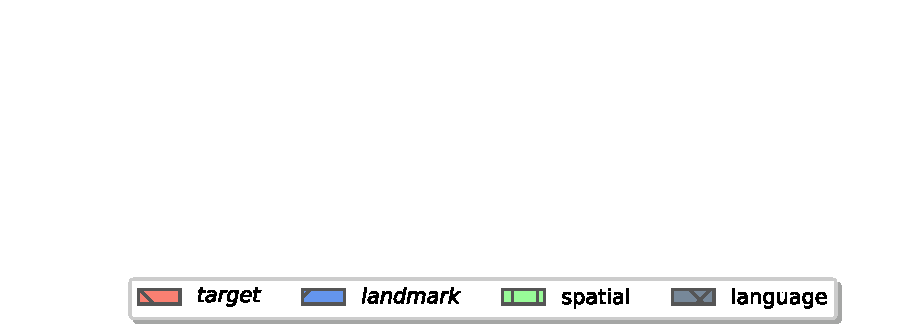
\includegraphics[width=0.9\columnwidth]{studies/inlg2019/figures/results/attentions/models/legend.pdf}\\
	\end{minipage}%
	\caption{The overall average of $\bm{\beta}$ on tokens of each semantic role (target, relation, landmark) on all examples of the test dataset, for 6 variations of the top-down knowledge about regions of interest (ROI): location of objects and their order as target and landmark.} 
	\label{inlg2019:fig:attention_roles}
\end{figure}

\begin{figure}[ht!]
	\centering
	\begin{minipage}{0.85\linewidth}
		\centering
		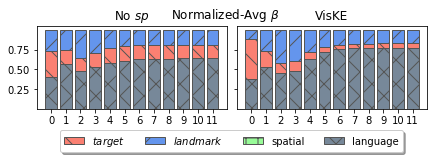
\includegraphics[width=\columnwidth]{studies/inlg2019/figures/results/attentions/random_all.png}\\
		(a)
	\end{minipage}\\
	\begin{minipage}{0.85\linewidth}
		\centering
		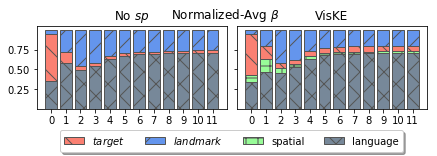
\includegraphics[width=\columnwidth]{studies/inlg2019/figures/results/attentions/order_all.png}\\
		(b)
	\end{minipage}%
	\caption{The average of $\bm{\beta}$ attentions of top-down models over sequences of words 1\ldots 11 (a) comparing $td$ and $td+VisKE$ and (b) comparing $td~order$ and $td~order+VisKE$. %
	} %
	\label{inlg2019:fig:attention_trend}
\end{figure}


\paragraph{Discussion}
The comparison of 6 models in Figure~\ref{inlg2019:fig:attention_roles} shows
that geometric $mask$ $\bm{s}$-features are not contributing as well
as dense $VisKE$ $\bm{s}$-features. %
In the models without top-down semantic role assignment %
only the model with $+VisKE$ features has the expected attention on
target and landmark, but there is no attention on the
$\bm{s}$-features.  In the models with top-down semantic role
assignment, the model with $VisKE$ $\bm{s}$-features has higher
attention on $\bm{s}$-features when predicting a relation word (H1). A
similar situation is observable over word sequences in
Figure~\ref{inlg2019:fig:attention_trend}. Without prior semantic role
assignment the model is more confused how to attend target or landmark
(H2). Finally, note that %
geometric $VisKE$ $\bm{s}$-features help predicting the
\textsc{target}-\textsc{landmark} roles when these are not assigned
top-down. %







\section{Related Work}
\label{inlg2019:sec:related_works}




\paragraph{Generating referring expressions}
Generating locative expressions is part of the general field of generating referring expressions \cite{DaleReiter:1995,Krahmer:2011aa} with applications such as describing scenes \cite{Viethen:2008aa} and images \cite{Mitchell:2012aa}.
The research on describing visible objects \cite{mitchell-etal-2013-generating} and human-robot dialogue \cite{kelleher-kruijff-2006-incremental} raised question about grounding relations in hierarchical representation of context.
Application of neural language models and using convolutional neural networks for encoding visual features is an open question in interactive GRE tasks.

\paragraph{Encoder-decoder models with attention} Recently several
methods focused on finding better neural architectures for generating
image descriptions based on pre-trained convolutional neural networks
have been introduced. \citet{karpathy2015deep} align descriptions with
images. \citet{vinyals2015show} introduce an encoder-decoder
framework. \citet{xu2015show} improve this approach with spatial
attention. \citet{lu2017knowing} introduce adaptive attention that
balances language and visual embeddings. The attention measure
provides an explanation of encoder-decoder architectures on how each
modality contributes to language generation. Based on the attended features
the %
performance of these models can be examined
\cite{liu2017attention,ghanimifard2018knowing}. In our paper, we
develop a model similar to the adaptive attention
which %
exploits its expressive aspects as 
a degree of 
grounding
in different features.

\paragraph{Outputs of external models as top-down features} In another
line of work, the output of the bottom-up visual understanding is used
as top-down features for language generation. For example, an object
detection pipeline is combined explicitly with language
generation. This procedure was previously used in template-based
language generation \cite{elliott2013image,elliott2015describing}. There have been
attempts to combine this process with neural language models with
attention. For example, \citet{you2016image} extract candidate
semantic attributes from images (e.g. a list of objects in the scene),
then the attention mechanism is used to learn to attend
on %
them when generating tokens of image descriptions.  Instead of
semantic attributes, \citet{anderson2018bottom} use a region proposal
network from a pre-trained object detection model to extract the
generated bounding box regions as possible locations of visual
clues. Then, the attention model learns to attend on the visual
features associated with these regions. The idea of using an object
detection module is also used in \citet{johnson2016densecap} %
where Faster R-CNN \cite{ren2015faster} is used to find regions of
interest. Instead of assigning one object class to each region, a full
description is generated for each proposed region.  In all of these
models, an image understanding module extracts some proposed
representations and then this knowledge is used as a top-down
representation of the scene to generate an image description.  In this
paper, we investigate the extent to which different spatial
information is facilitating as a top-down knowledge to generate
descriptions of scenes with neural language
models. %

\paragraph{Modular design} %
Our paper examines strategies that can demonstrate 
language grounding within a neural architecture. The studies of neural
architectures such as \cite{tanti2018put} provide analytical insight
on differences between multimodal architectures for language
generation.  
The modular design is mostly used in language parsing
tasks such as \cite{hu2017modeling} where object recognition,
localisation and relation recognition are separate modules for
grounding different parts of image descriptions in images in order to
solve tasks such as visual question answering.  In our paper, the
modularity of the neural architecture is not focused on parsing text
but used to incrementally demonstrate the contribution of each
introduced modality to language generation.

\paragraph{Multimodal embeddings} %
There are related studies on learning multimodal embeddings
\cite{kiros2014multimodal,lazaridou2015combining} to represent vision
and language in the same semantic space.  The focus of our paper is
to investigate how these different modalities complement each other in
neural language generation. In our models, the semantic
representations of spatial relations are considered as a separate
modality extending both the language and visual embeddings.  There are
related studies on encoding spatial knowledge in feature space in
order to predict spatial prepositions \cite{ramisa2015combining} or on
prepositional embeddings which can predict regions in space
\cite{collell2018learning}.  In our paper, we investigate the degree
in which each embedding contributes to language generation within the
neural language model.



\section{Conclusions}\label{inlg2019:sec:conclusion}



We explored the effects of encoding top-down spatial knowledge in a
bottom-up trained generative neural language model for the image
description task.
The findings of the experiments in this paper are as follows:


(1)
 Overall, integration of top-down knowledge has a positive
  effect on grounded neural language models for this
  task. %
(2)
 When combining bottom-up language grounding with top-down
  knowledge representation as different features, different types of
  top-down knowledge have different contribution to grounded language
  models. The general picture is further complicated by the fact that
  different spatial relations have different bias to different
  knowledge.
(3)
 The performance gain from the geometric features extracted
  from bounding boxes ($\bm{s}$-features) is smaller than initially
  expected, with two possible explanations related to the nature of
  the corpora of image descriptions: (i) The corpus contains images of
  typical scenes where the relation of objects with each other is
  predictable from the description and therefore is captured in the
  language model; (ii) As annotators are focused on describing ``what
  is in the image'' rather ``where things are spatially in relation to
  each other'', descriptions of geometric spatial relations which
  refer to the locational information are rare in the corpus.
(4)
 The majority of attention is placed on the language model
  which demonstrates that this provides significant information when
  generating spatial descriptions. While this may be a confounding
  factor if the visual features are ignored, the language model also
  encodes useful information about spatial information as discussed in
  \cite{kulkarni2011baby,dobnik-etal-2018-exploring}.


The results open several questions about grounded language
models. Firstly, the degree to which the system is using each modality
can be affected by dataset biases and this should be taken into
account in the forthcoming work. Given this bias, learning a single
common language model for descriptions of spatial scenes is
insufficient as different kinds of knowledge may come to focus in
different interactional scenarios. This further supports the idea that
top-down integration of knowledge is required where we hope that the
models will learn to attend to the appropriate features.  Secondly,
our investigation leaves open the question whether the representations
both visual and geometric that we use are good representations for
learning spatial relations. Further work will include a focused
investigation of what kind of geometric relations they encode.






\section*{Acknowledgements}

The research reported in this paper was supported by a grant from the
Swedish Research Council (VR project 2014-39) for the establishment of
the Centre for Linguistic Theory and Studies in Probability (CLASP) at
the University of Gothenburg.



\section{Appendix: Model Details}
\label{appendix:models}
\paragraph{Generative language model}
We use a simple forward recurrent neural model with cross-entropy loss in all model variations:
\begin{align}\label{inlg2019:eq:lm}
P(w_{t+1} | w_{0:t}, c) &= \hat{\bm{y}}_{t+1} = \bm{F}(w_{0:t}, c; \theta) \\
loss(k_{1:t},\theta) &= -\sum_{t=0}^{T}\mathrm{log}(\bm{\delta_{k_t}} \cdot \hat{y}_{t})
\end{align} 
\noindent where $\bm{F}$ represents the neural network function with parameters $\theta$, inputs $w_{0:t}$ the sequence of words with $w_0$ the sentence marker `$\langle$s$\rangle$', and $c$ to represent the image or with additional top-down knowledge. 
$\hat{y}_{t+1} \in [0,1]^{|V|}$ is a categorical distribution over the choices in vocabulary $V$ for the conditional probability of the next word. 
The loss is calculated for each sample of word sequence $[v_{k_{0}}, v_{k_{1}}, ...,v_{k_{T}}]$, which $k_t \in \{1,...|V|\}$ refers to the word index in the vocabulary, and $\delta_{k_t}$ is its one-hot encoding.

\paragraph{Simple encoder-decoder} An encoder-decoder architecture without spatial attention, similar to \cite{vinyals2015show}, is the most simple baseline for setting up the experiments and designing the foundation for fusing vision and language. 
The input to the model is an image and the start symbol $<s>$ for the language model decoder. 
The word embeddings $e_t$ are concatenated with the scene visual features ($\bar{\bm{v}}$).
The embeddings are randomly initialised and learned as a parameter set for the model.
The visual vectors are produced by a pre-trained ResNet50 \cite{he2016deep}.
Then, $\bar{\bm{v}}$ is made by a dense layer translating the visual vector to a unified tensor size for computational convenience.
This layers also helps fine-tuning the visual features. 
\begin{align*}
F_v(\bm{x}) = \mathrm{ReLU}(\bm{W}_v \cdot \bm{x} + \bm{b}_v) \\
\bar{\bm{v}} = \frac{\sum_{i=1}^{k}{F_v(\bm{v}^{\prime}_i)}}{k}
\end{align*}
\noindent where $F_v$ the function in Figure~\ref{inlg2019:fig:visual_finetune_a}, $\bm{v}^{\prime}_i \in \mathbb{R}^{2048}$ with ResNet50 dimensions, $\bm{W}_v \in \mathbb{R}^{100 \times 2048}$ and  $\bm{b}_v \in \mathbb{R}^{100}$ are parameters to be learned as fine-tuning.
The resulting vector is concatenated to a word embedding and fed to the Long-Short Term Memory (LSTM) network \cite{hochreiter1997long} and its output to a multi-layer perceptron (MLP) with a softmax layer which predicts the next word, as it was described earlier in Equation~\ref{inlg2019:eq:lm}. This function would be:
\begin{equation}
\hat{\bm{y}}_{t+1} = \textrm{softmax}(\mathrm{MLP}(\mathrm{LSTM}([\bm{e}_{t};\bar{\bm{v}}], \bm{h}_{t-1})))
\end{equation}
\noindent where $\bm{e}_{t}$ and $\bm{h}_{t}$ respectively represent the word embedding and the hidden unit in recurrent cell at time $t$ of the word sequence (Figure~\ref{inlg2019:fig:architectures}a). Ideally, the spatial features must be learned bottom-up in $\bar{\bm{v}}$ as other visual features in the deep layers of convolutions in ResNet.


\paragraph{Adaptive attention}
The simple encoder-decoder architecture relies on bottom-up learning of visual features and geometric arrangement of objects.
However, it has been shown in recent image captioning models that a spatial attention mechanism to localise each word improves the language generation \cite{xu2015show}. 
Moreover, the attentions can be learned as an adaptation of modalities. 
Based on this assumption we will use the adaptive attention similar to \cite{lu2017knowing}.
In generalisation of adaptive attention, the feature vectors including visual features from different locations as well as the contextual language features and other modalities $\hat{\bm{f}} = [f_1, f_2, ..., f_n]$ are fused with weighted sum according to their attention weight $\hat{\bm{\alpha}}$. 
\begin{equation}
\hat{\bm{c}}_t = \sum_{i=1}^n \bm{\alpha}_{i} f_{i}
\end{equation}
\noindent where $\hat{\bm{c}}_t$ represents the fused vector after applying adaptive attention on $n$ feature vectors. Knowing which features in what degree contribute to prediction of the next word is decided in a multi-layer perceptron ($MLP_a$) with softmax as $\hat{\bm{\alpha}}$ in Figure~\ref{inlg2019:fig:attention}. %
This module is formalised in a sequential process as follows:
\begin{align*}
\bm{z}_t &= \bm{W}_{a}^2 \tanh(\bm{W}_{a}^1 \cdot \hat{\bm{f}}_t) \\
\hat{\bm{\alpha}}_t &= \textrm{softmax}(\bm{z}_t).
\end{align*}
\noindent where $\hat{\bm{\alpha}}_t = [\bm{\alpha}_{t,1}, \bm{\alpha}_{t,2}, ..., \bm{\alpha}_{t,n}]$ is the output of the module in time $t$, and $\bm{W}_{a}^1$,$\bm{W}_{a}^2$ are the parameters of the module which will be trained in the model.
\begin{figure}[ht!]
	\centering
	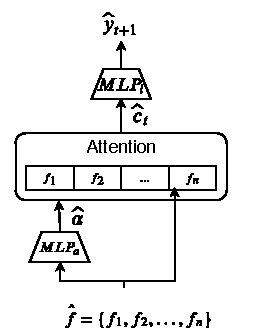
\includegraphics[width=0.3\linewidth]{studies/inlg2019/figures/merge_attention.pdf}
	\caption{The generalised adaptive attention module.}\label{inlg2019:fig:attention}
\end{figure}

\paragraph{Bottom-up localisation}
With visual feature representing each region of the image as in Figure~\ref{inlg2019:fig:visual_finetune_a}, attention mechanism is going to work as localisation model. %
We designed the interaction between the attention mechanism and the language model more similar to \cite{anderson2018bottom}: two layers of stacked LSTM, the first stack ($\mathrm{LSTM}_a$) to produce features for attention model, then the second stack ($\mathrm{LSTM}_l$) to produce contextualised linguistic features to be fused with attended visual features (Figure~\ref{inlg2019:fig:architectures}b).
This design makes it easier to be extended with top-down visual vectors.
\begin{equation}
\hat{\bm{c}}_t = \sum_{i=1}^{49} \bm{\alpha}_{t,i} \bm{v}_{i} + \bm{\alpha}_{t,50} {\bm{h}_t^l}
\end{equation}
\noindent where each $\bm{v}_{i}$ is a visual feature referring to one of the 49 locations in Figure~\ref{inlg2019:fig:visual_finetune_a}, and $\bm{h}_t^l$ is the contextualised language feature from $\mathrm{LSTM}_l$. 


\paragraph{Top-down localisation}
Unlike the bottom-up localisation, the top-down method has a list of regions of interest pre-processed from other procedures. 
The process of region proposals can be part of a bottom-up process as in \citet{anderson2018bottom} or \citet{johnson2016densecap} which instead of the grids of regions in ConvNets in Figure~\ref{inlg2019:fig:visual_finetune_a} a Faster R-CNN \cite{ren2015faster} is used to extract all possible regions of interest. 
In this paper, we use the bounding box annotations on images as the top-down localisation knowledge, then we use ResNet50 to extract visual features from these regions Figure~\ref{inlg2019:fig:visual_finetune_b}.
At this stage the top-down visual representation only proposes visual vectors of two objects in random order without their spatial role in intended descriptions shown in Figure~\ref{inlg2019:fig:architectures}d.
\begin{equation}\label{inlg2019:eq:td}
\hat{\bm{c}}_t = \bm{\alpha}_{t,1} \bm{v}_{obj_1} + \bm{\alpha}_{t,2} \bm{v}_{obj_2} + \bm{\alpha}_{t,3} {\bm{h}_t^l}
\end{equation}
\noindent where each $\bm{v}_{obj_1}$ and $\bm{v}_{obj_2}$ are the visual features referring to two regions in Figure~\ref{inlg2019:fig:visual_finetune_b}, and $\bm{h}_t^l$ is the contextualised language feature from $\mathrm{LSTM}_l$. 


\paragraph{Top-down target-landmark assignment} 
Another top-down information is the assignment of one region as the target and another region as the landmark. 
This top-down knowledge is encoded as the order in the list of two object, first object is the target and the second object is the landmark in Equation~\ref{inlg2019:eq:td}. 
\begin{equation}
\hat{\bm{c}}_t = \bm{\alpha}_{t,1} \bm{v}_{\textsc{target}} + \bm{\alpha}_{t,2} \bm{v}_{\textsc{landmark}} + \bm{\alpha}_{t,3} {\bm{h}_t^l}
\end{equation}
\noindent where each $\bm{v}_{\textsc{target}}$ and $\bm{v}_{\textsc{landmark}}$ are the visual features referring to two regions in Figure~\ref{inlg2019:fig:visual_finetune_b} and their semantic role is defined top-down.


\paragraph{Top-down geometric features}
With top-down localisation we may lose the relative location of two objects since they are processed separately in two disconnected convolutional neural networks.
Therefore, the top-down geometric features are required for grounding of denotation of the locational words.
Additionally, representing geometric knowledge can encode the frame of reference. 
For example, a simple geometric relation between two bounding boxes can be an arrow from the centre of one bounding box to the centre of the other, however the choice between the order of objects depends on the frame of reference (i.e. $obj_1 \rightarrow obj_2$ or $obj_1 \leftarrow obj_2$). 
We represent the geometric features by considering the top-down target-landmark assignment (i.e. $\textsc{target} \rightarrow \textsc{landmark}$). 
Therefore with these feature vectors we encode the top-down frame of reference as well.
This creates different variations of feature fusions (Table~\ref{inlg2019:tab:models2}).

\begin{table*}[htb]
	\centering
	\scriptsize
	\begin{tabular}{|l|l|l|}
		\hline
		Model name   & Visual features & Attention \\
		\hline
		$bu49$       & $[\bm{v}_{1}, ..., \bm{v}_{49}]$ & $\hat{\bm{c}}_t = \sum_{i=1}^{49} \bm{\alpha}_{t,i} \bm{v}_{i} + \bm{\alpha}_{t,50} {\bm{h}_t^l}$
		\\
		$bu49+mask$  & $[\bm{v}_{1}, ..., \bm{v}_{49}]$ & $\hat{\bm{c}}_t = \sum_{i=1}^{49} \bm{\alpha}_{t,i} \bm{v}_{i} + \bm{\alpha}_{t,50} {\bm{h}_t^l} + \bm{\alpha}_{t,51} \bm{s}$ \\
		$bu49+VisKE$ & $[\bm{v}_{1}, ..., \bm{v}_{49}]$ & $\hat{\bm{c}}_t = \sum_{i=1}^{49} \bm{\alpha}_{t,i} \bm{v}_{i} + \bm{\alpha}_{t,50} {\bm{h}_t^l} + \bm{\alpha}_{t,51} \bm{s}$ \\
		\hline
		$td$         & $[\bm{v}_{obj_1}, \bm{v}_{obj_2}]$ & $\hat{\bm{c}}_t = \bm{\alpha}_{t,1} \bm{v}_{\textsc{target}} + \bm{\alpha}_{t,2} \bm{v}_{\textsc{landmark}} + \bm{\alpha}_{t,3} {\bm{h}_t^l}$ \\
		$td+mask$    & $[\bm{v}_{obj_1}, \bm{v}_{obj_2}]$ & $\hat{\bm{c}}_t = \bm{\alpha}_{t,1} \bm{v}_{obj_1} + \bm{\alpha}_{t,2} \bm{v}_{obj_2} + \bm{\alpha}_{t,3} {\bm{h}_t^l} + \bm{\alpha}_{t,4} \bm{s}$ \\
		$td+VisKE$   & $[\bm{v}_{obj_1}, \bm{v}_{obj_2}]$ & $\hat{\bm{c}}_t = \bm{\alpha}_{t,1} \bm{v}_{obj_1} + \bm{\alpha}_{t,2} \bm{v}_{obj_2} + \bm{\alpha}_{t,3} {\bm{h}_t^l} + \bm{\alpha}_{t,4} \bm{s}$ \\
		\hline
		$td~(order)$ & $[\bm{v}_{\textsc{target}}, \bm{v}_{\textsc{landmark}}]$ & $\hat{\bm{c}}_t = \bm{\alpha}_{t,1} \bm{v}_{\textsc{target}} + \bm{\alpha}_{t,2} \bm{v}_{\textsc{landmark}} + \bm{\alpha}_{t,3} {\bm{h}_t^l}$ \\
		$td+mask~(order)$ & $[\bm{v}_{\textsc{target}}, \bm{v}_{\textsc{landmark}}]$ & $\hat{\bm{c}}_t = \bm{\alpha}_{t,1} \bm{v}_{\textsc{target}} + \bm{\alpha}_{t,2} \bm{v}_{\textsc{landmark}} + \bm{\alpha}_{t,3} {\bm{h}_t^l} + \bm{\alpha}_{t,4} \bm{s}$ \\
		$td+VisKE~(order)$ & $[\bm{v}_{\textsc{target}}, \bm{v}_{\textsc{landmark}}]$ & $\hat{\bm{c}}_t = \bm{\alpha}_{t,1} \bm{v}_{\textsc{target}} + \bm{\alpha}_{t,2} \bm{v}_{\textsc{landmark}} + \bm{\alpha}_{t,3} {\bm{h}_t^l} + \bm{\alpha}_{t,4} \bm{s}$ \\
		\hline
	\end{tabular}
	\vspace{0.5em}
	\caption{The visual features and their attention}
	\label{inlg2019:tab:models2}
\end{table*}

In order to find the best encoding of top-down geometric features, we considered two different vectorisation strategies to represent relation between two bounding boxes Figure~\ref{inlg2019:fig:spatial}.
\begin{itemize}[noitemsep]
	\item ($mask$) a concatenation of two mask vectors in 49 locations (Figure~\ref{inlg2019:fig:spatial}a).
	\item ($VisKE$) a dense representation with 11 geometric features according to \cite{sadeghi2015viske}  (Figure~\ref{inlg2019:fig:spatial}b): where $dx, dy$ are changes in coordinates of the centres, $ov, ov_1, ov_2$ the overlapping areas (total, relative to the first, and the second bounding box), $h_1, h_2$ heights, $w_1, w_2$ widths and $a_1, a_2$ areas.
\end{itemize}
Then, a feed-forward network with two layers ($F_s$) is used to project geometric features into a 100-dimension vector to become comparable with other modalities. %
\begin{align*}
F_s(\bm{x}) &= \bm{W}_{s}^2 \tanh(\bm{W}_{s}^1 \cdot \bm{x} + \bm{b}_{s}^1) \\
\bm{s} &= F_s(\bm{s}')
\end{align*}
\noindent where $\bm{s}$ represents the transformed geometric spatial features, and $\bm{W}_{s}^2 \in \mathbb{R}^{100 \times 100}, \bm{W}_{s}^1 \in \mathbb{R}^{100 \times 11} (or~\mathbb{R}^{100 \times 98})$ are the set parameters regarding this module to be learned in the model. 



\section{Examples of generated descriptions}
\label{appendix:generations}
More examples of generated descriptions with beam search of depth $5$ are shown in Figure~\ref{inlg2019:fig:data_example2a}. 
\begin{figure*}[hb]
	\begin{minipage}{\textwidth}
		\centering
		\begin{minipage}{0.3\textwidth}
			\centering
			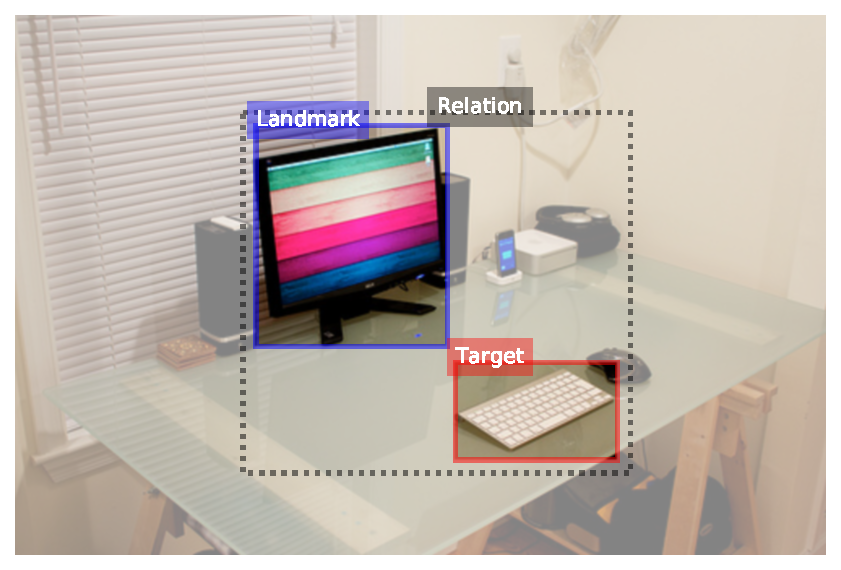
\includegraphics[scale=0.25]{studies/inlg2019/figures/2413204_keyboard_in_front_of_computer.pdf}
		\end{minipage}%
		\begin{minipage}{0.7\textwidth}%
			\begin{tabular}{|ll}
				\multicolumn{2}{|l}{$\langle$ ``{\color{red} keyboard}", ``in front of", ``{\color{blue} computer}"$\rangle$} \\
				$simple$         & {computer} \\
				$bu49$           & {keyboard~on~desk} \\
				$td$             & {computer~on~top~of~desk} \\
				$td~order$       & {keyboard~on~computer} \\
				$td~order+VisKE$ & {keyboard~on~computer} \\
			\end{tabular}%
		\end{minipage}\\
		\rule{\textwidth}{0.5pt}
		\begin{minipage}{0.3\textwidth}
			\centering
			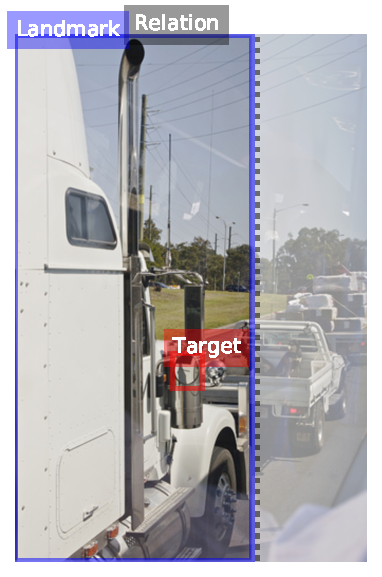
\includegraphics[scale=0.3]{studies/inlg2019/figures/2417890_mirror_on_side_of_semi.pdf}
		\end{minipage}%
		\begin{minipage}{0.7\textwidth}%
			\begin{tabular}{|ll}
				\multicolumn{2}{|l}{$\langle$ ``{\color{red} mirror}", ``in side of", ``{\color{blue} semi}"$\rangle$} \\
				$simple$         & {truck} \\
				$bu49$           & {truck~has~door} \\
				$td$             & {door~on~truck} \\
				$td~order$       & {light~on~road} \\
				$td~order+VisKE$ & {mirror~on~truck} \\
			\end{tabular}
		\end{minipage}\\
		\rule{\textwidth}{0.5pt}
		\begin{minipage}{0.3\textwidth}
			\centering
			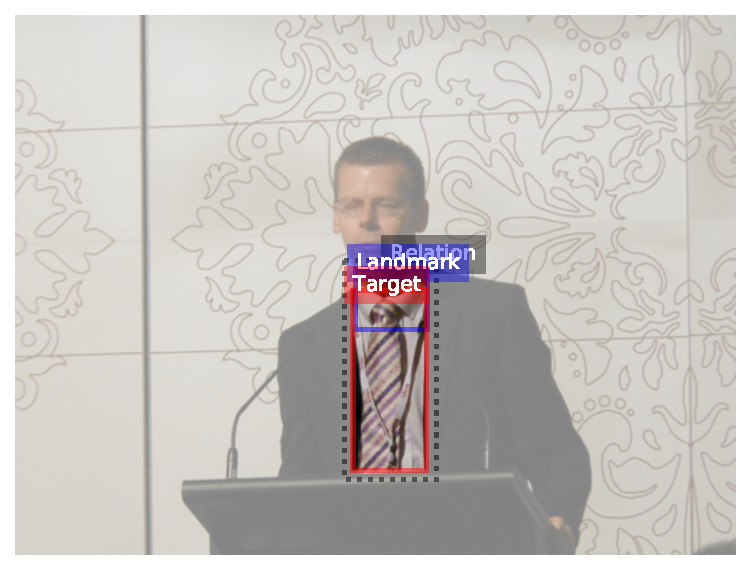
\includegraphics[scale=0.25]{studies/inlg2019/figures/2413371_lanyard_around_neck.pdf}
		\end{minipage}%
		\begin{minipage}{0.7\textwidth}%
			\begin{tabular}{|ll}
				\multicolumn{2}{|l}{$\langle$ ``{\color{red} lanyard}", ``around", ``{\color{blue} neck}"$\rangle$} \\
				$simple$         & {tie} \\
				$bu49$           & {man~has~hair} \\
				$td$             & {tie~around~neck} \\
				$td~order$       & {tie~around~neck} \\
				$td~order+VisKE$ & {tie~around~neck} \\
			\end{tabular}	
		\end{minipage}%
		\caption{From VisualGenome:
			2413204\protect\footnote{\citet{vg2413204}: CC BY-NC-SA 2.0.}
			2417890\protect\footnote{\citet{vg2417890}: CC BY-NC 2.0.}
			2413371\protect\footnote{\citet{vg2413371}: CC BY-SA 2.0.}
		}\label{inlg2019:fig:data_example2a}
	\end{minipage}%
\end{figure*}


\clearpage
\bibliographystyle{acl_natbib}
\bibliography{studies/inlg2019/references.bib}
